% This template was initially provided by Dulip Withanage.
% Modifications for the database systems research group
% were made by Conny Junghans,  Jannik Strötgen and Michael Gertz

\documentclass[
     12pt,         % font size
     a4paper,      % paper format
     BCOR10mm,     % binding correction
     DIV14,        % stripe size for margin calculation
%     liststotoc,   % table listing in toc
%     bibtotoc,     % bibliography in toc
%     idxtotoc,     % index in toc
%     parskip       % paragraph skip instad of paragraph indent
     ]{scrreprt}

%%%%%%%%%%%%%%%%%%%%%%%%%%%%%%%%%%%%%%%%%%%%%%%%%%%%%%%%%%%%

% PACKAGES:

% Use German :
\usepackage[ngerman]{babel}
% Input and font encoding
\usepackage[utf8]{inputenc}
\usepackage[T1]{fontenc}
% Index-generation
\usepackage{makeidx}
% Einbinden von URLs:
\usepackage{url}
% Special \LaTex symbols (e.g. \BibTeX):
%\usepackage{doc}
% Include Graphic-files:
\usepackage{graphicx}
% Include doc++ generated tex-files:
%\usepackage{docxx}
% Include PDF links
%\usepackage[pdftex, bookmarks=true]{hyperref}

% Fuer anderthalbzeiligen Textsatz
\usepackage{setspace}
\usepackage{amsmath}
% hyperrefs in the documents
\usepackage[bookmarks=true,colorlinks,pdfpagelabels,pdfstartview = FitH,bookmarksopen = true,bookmarksnumbered = true,linkcolor = black,plainpages = false,hypertexnames = false,citecolor = black,urlcolor=black]{hyperref} 
%\usepackage{hyperref}

%%%%%%%%%%%%%%%%%%%%%%%%%%%%%%%%%%%%%%%%%%%%%%%%%%%%%%%%%%%%

% OTHER SETTINGS:

% Pagestyle:
\pagestyle{headings}

% Choose language
\newcommand{\setlang}[1]{\selectlanguage{#1}\nonfrenchspacing}


\begin{document}

% TITLE:
\pagenumbering{roman} 
\begin{titlepage}


\vspace*{1cm}
\begin{center}
\vspace*{3cm}
\textbf{ 
\Large Heidelberg University\\
\smallskip
\Large Data and Computer Science\\
\smallskip
}

\vspace{3cm}

\textbf{\large Master-Arbeit} % Bachelor-Arbeit 

\vspace{0.5\baselineskip}
{\huge
\textbf{Research and Development of NMOps (Numerical Model Operations)}
}
\end{center}

\vfill 

{\large
\begin{tabular}[l]{ll}
Name: & Keerthan Ugrani\\
Matrikelnummer: & 3770219\\
Betreuer: & Prof. Dr. Ekaterina Kostina, Prof. Dr. Nima, 
\\ & and Shuldham Peard\\
Datum der Abgabe: & \today
\end{tabular}
}

\end{titlepage}

\onehalfspacing

\thispagestyle{empty}

\vspace*{100pt}
\noindent
Ich versichere, dass ich diese Master-Arbeit selbstständig verfasst und nur die angegebenen
Quellen und Hilfsmittel verwendet habe und die Grundsätze und
Empfehlungen ``Verantwortung in der Wissenschaft'' der Universität Heidelberg beachtet wurden. 

\vspace*{50pt}
\noindent

\underline{\phantom{mmmmmmmmmmmmmmmmmmmm}}

\medskip
\noindent 
Abgabedatum: \today
\newpage

% Add a brief summary of your topic and contributions (Zusammenfassung) in German *and* in English:
\chapter*{Zusammenfassung}

% This file contains the German version of your abstract, with about 300-500 words

Die Zusammenfassung muss auf Deutsch \textbf{und} auf Englisch geschrieben
werden. Die Zusammenfassung sollte zwischen einer halben und einer
ganzen Seite lang sein. Sie soll den Kontext der Arbeit, die
Problemstellung, die Zielsetzung und die entwickelten Methoden sowie
Erkenntnisse bzw.~Ergebnisse übersichtlich und verständlich
beschreiben.
\newpage

\chapter*{Abstract}

% This file contains an abstract of your thesis, with approximaltely 300-500 words

Battery Management System (BMS) plays a crucial role in monitoring and maintaining the performance and health of the batteries, particularly in electric vehicles and energy storage applications. Accurate prediction of SoH (State of Health) and SoC (State of Charge) is essential for sustainable approach. Semi-empirical models, which combine physical principles with empirical data, are highly effective for such estimations but present significant challenges in terms of stability, real-time deployment, and continuous feedback. While Machine Learning Operations (MLOps) has matured for ML models, there is no equivalent framework for managing, deploying and scaling semi-empirical models. Conventional SoH semi-empirical models, while grounded in electro-chemical principles, exhibit limited adaptability due to their reliance on fixed parameterization, inability to generalize across varying operating conditions, and lacks scalability. These models often deviate from the test-bench SoH measurements, leading to sub-optimal SoH predictions in real-world applications. 

This research develops a Numerical Model Operations (NMOps) architecture follows a MLOps architecture, enabling management, deployment and scaling of semi-empirical models, or otherwise any numerical hybrid models. Moving Horizon Estimation (MHE) is employed as the core algorithm in this architecture to compute an optimal correction factor that aligns semi-empirical SOH estimates with laboratory derived test-bench SOH under equivalent degradation conditions. The MHE correction factor is optimized using a regularized least-squares minimization approach over a finite horizon, ensuring smooth and stable parameter adjustments. Extended Kalman Filter (EKF) is subsequently applied to refine the corrected SOH estimates by reducing transient fluctuations and measurement noise, ensuring robust time-series consistency.

Validation is conducted through statistical metrics such as Root Mean Sqaure Error (RMSE), Mean Absolute Percentage Error (MAPE),and Pearson Correlation Coefficient, ensuring that SOH estimates exhibit high fidelity to test bench ground truth data. ("results and conclusion to be updated").

\newpage

% MAIN PART:
% Table of contents (Inhaltsverzeichnis)
\tableofcontents
\cleardoublepage
\pagenumbering{arabic} 

% List of figures (Abbildungsverzeichnis):
%\listoffigures
% List of tables (Tabellenverzeichnis):
%\listoftables

%%%%%%%%%%%%%%%%%%%%%%%%%%%%%%%%%%%%%%%%%%%%%%%%%%%%%%%%%%%%%%%
% Here, the actual content of your thesis begins
% You can either put all the text here or use individual files to store the chapters of your thesis.
% Below are templates for both alternatives.

\chapter{Introduction}\label{intro}

% This file contains Introduction of the thesis

A Battery Management System is a vital electronic control system that monitors, manages, and protects battery packs to ensure safe and efficient operations \cite{wevj-12-00120-v2}. A battery pack comprises numerous cells linked either in series or parallel, each possessing distinct traits that require oversight and adjustment to boost durability and cut costs \cite{energies-18-00342-v2}\cite{wevj-12-00120-v2}. Apart from the cells themselves, certain threshold, must be maintained to extend their operational life. These threshold include temperature ranges, charge and discharge rates, current termination points, and upper/lower voltage boundaries. Integrated within the battery pack is a system known as Battery Management System (BMS). A proficient BMS safeguards the battery from physical wear and tear, forecasts its longevity, controls the charge-discharge cycles, and impacts the total life cycles. Its key tasks involve tracking cell heat levels, managing thermal conditions, equalizing cell voltages, measuring current across modules or the pack, calculating state of charge (SOC) and state of health (SOH), and fine-tuning cells to slow degradation. Consequently, an effective BMS improves battery supervision, ensures secure functioning, provides maximum power output, and lengthens service life. It also needs to coordinate with onboard components—such as the motor controller, climate regulator, shared bus, diagnostic system, and vehicle processor—to carry out diverse operations \cite{wevj-12-00120-v2}. 

In Electric Vehicles (EVs), the BMS has to perform pretty complex tasks due to the complicated nature of the batteries, such as high capacity, high power, wide temperature variation and harsh driving conditions. The accurate estimation of state variables such as State of Charge (SOC) and State of Health (SOH) is pivotal in the management of Lithium-Ion batteries \cite{105207_1_5.0172683}. These variables provide essential information about the status and overall health of the battery, which is fundamental for optimal battery management \cite{105207_1_5.0172683}. Correctly predicting battery SOH plays a crucial role in extending the lifespan of new energy vehicles, ensuring their safety, and promoting their sustainable development\cite{electronics-13-01675}. 

Some of the key functionalities and features of a BMS:
\begin{itemize}
    \item \textbf{State of Charge (SOC) Estimation:} Describes a battery’s remaining capability as a proportion of the total capacity under the same conditions\cite{wevj-12-00120-v2}. Accurate SOC estimation is very important to monitor and optimize the performance of the batteries by controlling their charging and discharging, and it can tell how long an EV can drive before charging.
    \item \textbf{State of Health (SOH) Estimation:} Provides the health condition of the batteries, i.e., their degree of degradation\cite{wevj-12-00120-v2}. It basically represents how many cycles are left before the battery will reach its end of life. Accurate SOH estimation is crucial for safe and reliable operation.
    \item \textbf{Cell Monitoring:} Continuously monitors the cell's conditions which will ultimately help in managing, protecting, equalizing, and controlling the operations \cite{wevj-12-00120-v2}.
    \item \textbf{Cell Balancing:}\cite{wevj-12-00120-v2} Tries to maintain an equal state of charge in each cell . This is a crucial task as even cells of the same model and manufacturer are not identical, and imbalance can reduce overall pack capacity and cause malfunction. Cell balancing topologies can be categorized as active and passive. Active cell balancing exploits all the stored energy, while passive balancing dissipates energy from high SOC cells. 
    \item \textbf{Thermal Management:} Screens the cell temperature and performs thermal management to avoid speedy degradation of the battery\cite{wevj-12-00120-v2}. Maintaining a uniform temperature distribution is essential for optimal battery operation, and BMS often incorporates Battery Thermal Management Systems (BTMS). Cooling systems can be internal or external \cite{energies-18-00342-v2}. 
    \item \textbf{Voltage Management:} Precisely measures the voltage of each cell using voltage acquisition channels. SOC estimation also depends heavily on voltage measurements \cite{wevj-12-00120-v2}. 
    \item \textbf{Current Measurement:}\cite{wevj-12-00120-v2} Acquires the current level of the battery pack.
    \item \textbf{Safety Features:} \cite{wevj-12-00120-v2} Provides protection against over- and undercurrent/voltage, overheating/pressure, leakage current/voltage, short circuits, over charging/discharging, faults in connected devices, ground faults, and system or command failures. 
    \item \textbf{Communication:} Maintains simultaneous bi-directional (internal and external) communications with the whole system (power electronics, vehicle control unit, etc.) to provide status updates, send/receive commands, and perform other functions in real time\cite{wevj-12-00120-v2}. 
    \item \textbf{Computation:} Performs many functions such as data collection, data processing, charging/discharging current control, and state estimations, requiring fast, dynamic, efficient, and accurate operation\cite{wevj-12-00120-v2}.
    \item \textbf{Data Monitoring and Storage:} Effectively monitors different parameters and has good data storage to utilize the stored data for various functions and hazard prediction\cite{wevj-12-00120-v2}.
    \item \textbf{Power Management Control:} Reduces power consumption and minimizes losses for safe, stable, and efficient operation\cite{wevj-12-00120-v2}.
    \item \textbf{Charging and Discharging Control:} Carefully monitors charging and discharging of cells as the efficiency, durability, and life cycle of LIB depend on it, ensuring operation within safe limits\cite{wevj-12-00120-v2}.
    \item \textbf{State of Power:}\cite{wevj-12-00120-v2} Indicates the battery's current power capability.
    \item \textbf{State of Safety (SOS):} Monitors and ensures the safety of the overall system considering changes in current, temperature, voltage, etc.\cite{wevj-12-00120-v2}.
    \item \textbf{Depth of Discharge (DOD):} Defines the percentage of the battery capability that has been discharged\cite{wevj-12-00120-v2}.
    \item \textbf{State of Function (SOF):} Determines how efficiently the battery can perform based on various parameters \cite{wevj-12-00120-v2}.
    \item \textbf{End of Discharge (EOD):} Refers to the stage when SOC is 0\% and the battery is empty \cite{wevj-12-00120-v2}.
    \item \textbf{Galvanic Isolation:} Provides isolation between high and low voltage sections for safety \cite{wevj-12-00120-v2}. 
\end{itemize}

The State of Health (SOH) is an important indicator of a lithium-ion battery's condition, reflecting the extent of its performance degradation compared to its initial state \cite{s41598-025-92262-8}. It provides essential information about the battery's overall health and is fundamental for optimal battery management \cite{105207_1_5.0172683}. Correctly predicting battery SOH plays a crucial role in extending the lifespan of new energy vehicles, ensuring their safety, and promoting their sustainable development \cite{electronics-13-01675}. An accurate SOH estimation provides critical insight into the battery's degradation process over time, enabling timely maintenance and replacement decisions, thereby preventing unexpected failures \cite{105207_1_5.0172683}.

Importance of Battery State of Health (SOH):
\begin{itemize}
    \item \textbf{Optimal Battery Management:} SOH information is fundamental for the efficient management of lithium-ion batteries \cite{105207_1_5.0172683}.
    \item \textbf{Lifespan Extension:} Accurate SOH prediction helps in formulating reasonable battery usage and maintenance plans, prolonging battery life \cite{electronics-13-01675}.
    \item \textbf{Safety Assurance:} Correctly predicting SOH ensures the safety of new energy vehicles \cite{electronics-13-01675}.
    \item \textbf{Timely Maintenance and Replacement:} SOH estimation enables timely decisions regarding battery maintenance and replacement, preventing unexpected failures \cite{105207_1_5.0172683}.
    \item \textbf{Remaining Useful Life (RUL) Prediction:} SOH estimation is often a precondition for estimating the battery's remaining useful life \cite{wevj-12-00120-v2}.
\end{itemize}

Definitions of SOH:
Currently, there are numerous definitions of battery SOH in the literature\cite{s41598-025-92262-8}. Mainstream evaluation methods typically rely on changes in capacity or internal resistance\cite{electronics-13-01675}.
\begin{itemize}
    \item \textbf{Capacity Based Definition:} The most widely used approach defines SOH based on the degree of capacity degradation \cite{s41598-025-92262-8}. It is calculated as the percentage of the current maximum available capacity ($Q_m$) of the battery in relation to its rated capacity ($Q_r$)\cite{electronics-13-01675}\cite{wevj-12-00113}: $$SOH = \frac{Q_m}{Q_r} \times 100\% \quad (1)$$ The change of capacity is directly related to the SOH of the battery, which can clearly and stably reflect the degradation process \cite{s41598-025-92262-8}. A battery is generally considered at the end of life (EOL) when its capacity has decreased to 80\% of its original value, as stated by IEEE standard 1188.1996\\ \cite{wevj-12-00113}\cite{energies-18-00342-v2}.
    \item \textbf{Internal Resistance Based Definition:}  SOH can also be defined according to the internal resistance of the battery\cite{wevj-12-00113}: $$SOH = \frac{R_e - R}{R_e - R_n} \times 100\% \quad (2)$$ where $R$ is the internal resistance under the current state, $R_e$ is the internal resistance of the battery when it reaches the end of life, and $R_n$ is the internal resistance of the new battery\cite{wevj-12-00113}. The increase of internal resistance is an important indicator of battery aging and contributes to the further decline of battery SOH\cite{wevj-12-00113}.
\end{itemize}

Relationship with other battery states:
\begin{itemize}
    \item \textbf{State of Charge (SOC):} Accurate assessment of battery cell capacity, which is reflected in the SOH, ensures timely replacement. Cell health (SOH) is evaluated by comparing initial and current capacity. The SOC is crucial for the SOH calculation\cite{energies-13-01811-v2}. Joint estimation of SOH and SOC is crucial, with capacity-based and resistance-based SOH estimation processes playing a significant role in updating SOC estimation\cite{energies-13-01811-v2}.
    \item \textbf{Remaining Useful Life (RUL):} SOH estimation is a precondition for estimating the battery's remaining useful life (RUL)\cite{wevj-12-00120-v2}. While some studies focus on RUL separately, most combine RUL and SOH, where SOH is predicted first, followed by RUL based on the SOH\cite{batteries-10-00181-v2}.
\end{itemize}

Factors affecting SOH:
The SOH of a lithium-ion battery is influenced by various factors that lead to degradation, including:
\begin{itemize}
    \item \textbf{Operating Conditions:} Current, temperature, depth of discharge (DOD), and state of charge (SOC) significantly impact battery aging\cite{energies-18-00342-v2}.
    \item \textbf{Cycling:} Charge and discharge cycles cause battery capacity to diminish over time, a process called degradation\cite{electronics-13-01675}\cite{batteries-10-00181-v2}. Overcharge and excessive discharge cycles negatively affect the SOH of batteries[]. Higher DOD often leads to greater internal resistances\cite{energies-18-00342-v2}. Cycling at very low (<25\%) or very high SOC (>90\%) can lead to more rapid degradation compared to moderate SOCs\cite{energies-18-00342-v2}. Temperature has a significant impact on performance degradation regardless of the electrode material\cite{energies-18-00342-v2}.
    \item \textbf{Calendar aging:} Degradation also occurs over time even when the battery is not actively used\cite{energies-18-00342-v2}.
    \item \textbf{Material Degradation:} Changes in battery electrodes and electrolytes contribute to the decline in SOH\cite{energies-18-00342-v2}.
\end{itemize}

As SOH estimation cannot be measured directly during normal operation that is, one cannot easily measure full capacity without fully discharging the battery. A variety of estimation techniques have been developed. There are three primary caegories of methods for estimating the SOH of lithium-ion batteries: model-based methods, datadriven methods, and hybrid (fusion) methods\cite{wevj-12-00113}. 
\begin{itemize}
    \item \textbf{Electrochemical Model-Based Estimation:} These approaches use physics-based electrochemical models of the battery to predict aging behavior. These methods rely on understanding the degradation  and failure mechanisms of lithium-ion batteries to estimate and predict SOH. These methods typically involve developing mathematical models that describe the battery's internal electrochemical and physical processes \cite{electronics-13-01675}\cite{s41598-025-92262-8}. The accuracy of the SOH estimation depends on how well the model's key parameters represent the internal aging of the battery \cite{wevj-12-00113}. Model-based methods for battery analysis offer several advantages, including their ability to provide detailed explanations of discharge behavior and underlying degradation mechanisms, with electrochemical models yielding valuable insights into the battery's internal state, while equivalent circuit models (ECMs) stand out for their simplicity and strong engineering practicality \cite{electronics-13-01675}\cite{wevj-12-00113}. However, these methods also face notable drawbacks, such as the complexity of many models, which involve numerous parameters that are challenging to identify accurately, and the susceptibility of ECM parameter accuracy to environmental changes, resulting in fluctuating outcomes and accumulating errors \cite{electronics-13-01675}\cite{wevj-12-00113}. Additionally, these approaches often incur high computational costs, restricting their use in real-time applications, and exhibit weak anti-interference capabilities in practical settings, where achieving high accuracy remains difficult. Furthermore, ECMs may overlook subtle factors influencing state-of-health (SOH) attenuation and fail to comprehensively address complex external stress variations, limiting their overall effectiveness \cite{electronics-13-01675}\cite{wevj-12-00113}.
    \item \textbf{Empirical Model-Based Estimation:} Empirical or equivalent-circuit models (ECM) are widely used in practice due to their simplicity \cite{energies-13-02825-v2}. In this method the battery is modeled as an electric circuit (combinations of voltage sources, resistors, capacitors) that imitates the battery's charge/discharge behavior. Agiging of the battery is reflected when there are changes in the model parameters. For instance, the battery's open circuit voltage curve, internal resistance or capacitance values. By tracking how these parameters drift over time, the BMS can infer SOH. Some of the generally used techniques involve estimation via filtering: the BMS uses algorithms like Kalman filters to recursively update model parameters (e.g., internal resistance increasing with age) based on measurements \cite{wevj-12-00113}. For example, an Extended Kalman Filter (EKF) or Unscented Kalman Filter (UKF) can be employed to jointly estimate the battery’s SOC and capacity (treating capacity as an unknown parameter that slowly changes) \cite{wevj-12-00113}. Empirical models are computationally lightweight and can be tuned to cell data, which is why most commercial BMS rely on them \cite{energies-13-02825-v2}. Their drawback is that they may not capture all failure modes; they rely on the assumption that past observed trends (e.g. capacity fade vs. cycle count) will continue, which might not hold under new conditions.
    \item \textbf{Data-Driven Methods:} Data-driven methods estimate SOH by analyzing data generated during battery operation, such as voltage, current, temperature, and charge-discharge duration, using artificial intelligence or statistical models \cite{wevj-12-00113}\cite{energies-13-01811-v2}\cite{electronics-13-01675}\cite{energies-13-02825-v2}.\\ These are often referred to as "black-box" models because they do not necessarily require an understanding of the internal physical or chemical reactions within the battery \cite{electronics-13-01675}. The relationship between measured parameters and SOH is learned from historical data \cite{wevj-12-00113}\cite{electronics-13-01675}. However, data-driven methods typically need large datasets of battery aging under various conditions for training, and their extrapolation beyond the training domain is not guaranteed. Ensuring robustness and interpretability of purely data-driven SOH estimates (especially in safety-critical applications like EVs) remains an area of active research.
    \item \textbf{Hybrid (fusion) Methods:}\cite{electronics-13-01675}\cite{energies-13-01811-v2} Hybrid (fusion) methods combine two or more different SOH estimation techniques, often integrating model-based and data-driven approaches, to improve accuracy, robustness, and reliability \cite{wevj-12-00113}. The aim is to leverage the strengths of different methods while compensating for their individual limitations.
\end{itemize}

\section{Motivation}
In this research we consider the semi-empirical model, which balances the computational efficiency and physics-based interpretability with respect to its optimization, scalability and lifecycle management. Though semi-empirical model balances computational efficiency and physics based modeling, they suffer from several key limitations that affect their reliability in dynamic operating environments. The following challenges motivate the need for an enhanced framework:
\begin{itemize}
    \item Semi-empirical models rely on fixed parameter sets, assuming gradual degradation behavior using historical data
    \item Assumption that battery degradation is influenced only by temperature variations, depth of discharge (DOD), charge/discharge cycles, and internal resistance.
    \item Fixed-parameter models do not adapt to real-world variations, leading to increasing SOH estimation errors over time.
    \item Existing semi-empirical models lack an automated feedback loop mechanism to validate SOH predictions against the test bench data.
    \item Model errors may accumulate over time, requiring manual recalibration.
    \item Current approaches manually tune correction factors for SOH estimation
    \item Semi-empirical models are not designed for cloud based inference.
    \item No real-time SOH monitoring framework exists for fleet-wide battery system.
    \item No structured validation pipeline is in place for tracking model performance over time.
\end{itemize}

\section{Objectives}
The primary objective of this research is to develop an automated, scalable, and adaptive SOH estimation framework that overcomes the limitations of traditional semi-empirical models. Specifically, this research aims to:
\begin{itemize}
    \item Design an adaptive SOH estimation model to compute the correction factor that updates SOH estimates without modifying the base model equations.
    \item Ensure real-time correction of SOH deviations observed in current SOH semi-empirical model.
    \item Develop an automated validation framework that continuously compares SOH estimates against equivalent test bench conditions.
    \item Implement filtering mechanism to refine transient fluctuations and sensor noise in corrected SOH predictions. 
    \item Develop an equivalent condition mapping strategy that aligns real-world SOH estimates with comparable test bench conditions.
    \item Use statistical trend matching to validate relative degradation rates instead of absolute SOH values.
\end{itemize}

\section{Structure of the Thesis}
This thesis is structured as follows:
\begin{itemize}
    \item \textbf{Chapter \ref{chap:grundlagen}: Fundamentals and Related Work} provides an overview of current semi-empirical SOH model, explore various correction methods, filtering approaches, and cloud-scale life-cycle management architecture.
    \item \textbf{Chapter \ref{chap:main}: My Contribution} details the design and implementation of the NMOps framework, including MHE and EKF integration.
    \item \textbf{Chapter \ref{chap:eval}: Experimental Evaluation} presents validation experiments comparing corrected SOH with test bench ground truth and analyzes hyperparameter tuning efficiency.
    \item \textbf{Chapter \ref{chap:concl}: Conclusion} summarizes key findings and discusses future research directions, including Neural ODE/PDE-based SOH modeling.
\end{itemize}


%%%%%%%%%%%%%%%%%%%%%%%%%%%%%%%%%%%%%%%%%%%%%%%%%%%%%%%%%%%%
\newpage

\chapter{Fundamentals and Related Works}
\label{chap:grundlagen}
In this chapter, we present the theoretical background and review existing literature relevant to developing and implementing the objectives outlined in Chapter~\ref{intro}. As established earlier, the accurate estimation of the State of Health (SOH) is critical for ensuring lithium-ion batteries' safety, reliability, and performance, particularly within electric vehicles (EVs) and large-scale energy storage systems. Reliable SOH estimation underpins effective maintenance strategies and helps avoid unexpected system failures, improving the overall operational lifecycle.

Existing SOH estimation methodologies can be broadly classified into four categories: direct measurement techniques, model-based approaches, data-driven methods, and hybrid models. Each class of methods offers trade-offs in terms of accuracy, complexity, interpretability, and computational demands. For real-world applications, especially those involving cloud-based Battery Management Systems (BMS), there is an increasing need for frameworks that support scalable, secure, and automated lifecycle management of these estimation models.

This chapter examines existing approaches' capabilities and limitations, focusing on semi-empirical models and their suitability for integrating modern, cloud-enabled infrastructures. We begin by outlining the foundational concepts of SOH modeling, followed by a critical analysis of the challenges associated with deploying semi-empirical models in dynamic, large-scale environments.

\section{Fundamentals of Battery Management System}

A Battery Management System (BMS) is the central control unit responsible for monitoring and maintaining lithium-ion batteries' performance, safety, and reliability. It performs a wide range of functions at the cell and pack level to ensure optimal operation throughout the battery's lifecycle. Key functionalities of a BMS include:

\begin{itemize}
    \item \textbf{State of Charge (SOC) Estimation:} Determines the remaining charge in the battery as a percentage of its total capacity under current conditions. This metric is crucial for estimating available driving range in electric vehicles and managing charging and discharging cycles \cite{wevj-12-00120-v2}.

    \item \textbf{State of Health (SOH) Estimation:} Evaluates the battery's condition relative to its original capacity, providing insight into aging and remaining useful life. Accurate SOH tracking is essential for reliable and safe operation \cite{wevj-12-00120-v2}.

    \item \textbf{Cell Monitoring:} Continuously observes key cell-level parameters such as voltage, temperature, and current, enabling real-time supervision and control\\ \cite{wevj-12-00120-v2}.

    \item \textbf{Cell Balancing:} Ensures uniform charge levels across all cells in the battery pack. Imbalances can cause premature capacity loss or system failure. Balancing strategies include passive (dissipative) and active (redistributive) methods \cite{wevj-12-00120-v2}.

    \item \textbf{Thermal Management:} Monitors cell temperatures and activates thermal control mechanisms to prevent overheating. Uniform temperature distribution is crucial for avoiding accelerated degradation. Thermal control can be implemented through internal or external cooling systems\\ \cite{wevj-12-00120-v2,energies-18-00342-v2}.

    \item \textbf{Voltage and Current Sensing:} Precisely measures individual cell voltages and pack current, integral to SOC and SOH estimations and safety monitoring \cite{wevj-12-00120-v2}.

    \item \textbf{Safety Management:} Detects and mitigates hazardous conditions such as overvoltage, undervoltage, overcurrent, short circuits, thermal runaway, and system-level faults \cite{wevj-12-00120-v2}.

    \item \textbf{Communication Interface:} Facilitates real-time data exchange between the battery and other vehicle or system components (e.g., power electronics, vehicle control units), enabling coordinated system-level control \cite{wevj-12-00120-v2}.

    \item \textbf{Computational Capabilities:} Executes core BMS algorithms, including estimation, diagnostics, and control logic, often requiring high-speed and accurate computation \cite{wevj-12-00120-v2}.

    \item \textbf{Data Logging and Storage:} Records operational metrics for performance analysis, fault detection, and predictive maintenance \cite{wevj-12-00120-v2}.

    \item \textbf{Power Flow Regulation:} Manages energy input and output to minimize losses, improve efficiency, and support stable operation \cite{wevj-12-00120-v2}.

    \item \textbf{Charge/Discharge Control:} Oversees the charging and discharging process to maintain optimal efficiency, longevity, and safety boundaries \cite{wevj-12-00120-v2}.

    \item \textbf{State of Power (SOP):} Estimates the instantaneous power that can be safely delivered or absorbed by the battery \cite{wevj-12-00120-v2}.

    \item \textbf{State of Safety (SOS):} Continuously evaluates operational safety by tracking deviations in key variables such as voltage, temperature, and current\\ \cite{wevj-12-00120-v2}.

    \item \textbf{Depth of Discharge (DOD):} Represents the percentage of discharged capacity relative to the total capacity, used to evaluate usage patterns and aging\\ \cite{wevj-12-00120-v2}.

    \item \textbf{State of Function (SOF):} Indicates the battery’s ability to perform under given operational conditions by aggregating several internal state estimations\\ \cite{wevj-12-00120-v2}.

    \item \textbf{End of Discharge (EOD):} Refers to the point at which the battery has reached its minimum allowable SOC and can no longer provide useful power\\ \cite{wevj-12-00120-v2}.

    \item \textbf{Galvanic Isolation:} Provides electrical separation between high-voltage and low-voltage domains to ensure user and system safety \cite{wevj-12-00120-v2}.
\end{itemize}


\section{SOH Semi-Empirical Model}
A semi-empirical model captures the system's behavior through theoretical insights and empirical data. These models are often used in cases where fully theoretical or purely empirical approaches are insufficient. Here’s how the listed factors relate to the semi-empirical cyclic aging model:

\begin{itemize}
    \item \textbf{Temperature Factor}:
    \begin{equation}
        F_{T,cyc.charging}(T_{cell}) = e^{\left(-\frac{a}{T_{cell}} + b\right)} \quad \text{for} \quad T_{cell} \geq 293.15 \, \text{K}
    \end{equation}
    where:
    \begin{itemize}
        \item $T_{cell}$ is the cell temperature.
        \item $a$ and $b$ are constant co-efficients
    \end{itemize}

    \item \textbf{SOC factor}: 
    \begin{equation}
        F_{SoC,cyc}(SoC_{mean}) = a \cdot SoC_{mean}^2 - b \cdot SoC_{mean} + c
    \end{equation}
    where:
    $a$, $b$ and $c$ are constant co-efficients

    \item \textbf{DOD Factor}:
    \begin{equation}
        C_{l,\Delta DOD,cyc}(\Delta DOD) = a \cdot e^{b \cdot \Delta DOD} + \dot{c}
    \end{equation}
    where: 
    $a$, $b$ and $c$ are constant co-efficients.

    \item \textbf{Internal Resistance Factor}:
    \begin{equation}
        TripAging_{IR}(TripAging) = \left(\frac{a}{b}\right)^3 \cdot (c \cdot TripAging)^d
    \end{equation}
    where:
    $a$, $b$, $c$ and $d$ are constant co-efficients.
\end{itemize}

\section{Machine Learning Operations (MLOps) Framework}
\label{MLOPS}  

Machine Learning Operations (MLOps) refers to a set of practices and tools that enable the development, deployment, monitoring, and maintenance of machine learning models in scalable and automated environments. Within cloud-based Battery Management Systems (BMS), MLOps provides a systematic approach to managing the full lifecycle of SOH estimation models—from data acquisition to continuous validation—ensuring high performance, adaptability, and reliability under dynamic operating conditions.

\subsection*{MLOps for Automated Lifecycle Management}

An effective MLOps pipeline streamlines the end-to-end process of managing machine learning models. The following components constitute the key stages of such a framework:

\begin{itemize}
    \item \textbf{Data Ingestion:} Raw data from various sources—including sensor streams, historical logs, or simulated outputs—is systematically collected and ingested. Synthetic data generation or augmentation may be applied to improve dataset diversity and robustness.
    
    \item \textbf{Exploration and Validation:} This stage includes profiling the dataset to understand its structure, statistical distribution, and completeness. Validation checks are implemented to detect outliers, inconsistencies, or format violations, ensuring the integrity of downstream processes.
    
    \item \textbf{Data Cleaning:} Inaccurate or inconsistent entries are corrected, and relevant features are reformatted or normalized to align with modeling requirements.
    
    \item \textbf{Data Labeling:} Data instances are annotated with appropriate labels or categories, enabling supervised learning algorithms to associate input features with target outputs.
    
    \item \textbf{Data Splitting:} The dataset is partitioned into training, validation, and test subsets. This segregation supports unbiased model evaluation and reduces the risk of overfitting.
    
    \item \textbf{Model Training:} Machine learning algorithms are applied to the training dataset to construct predictive models. Feature engineering and hyperparameter tuning are integrated into this step to improve generalization performance.
    
    \item \textbf{Model Evaluation:} The trained model is assessed using the validation dataset to measure its performance against predefined metrics. This stage determines the model's readiness for deployment.
    
    \item \textbf{Model Testing:} Final validation is conducted using an unseen test dataset to verify model robustness and reliability before it is introduced into production.
    
    \item \textbf{Model Packaging:} The approved model is encapsulated into a standardized format—often with necessary metadata and dependencies—for integration with production systems.
    
    \item \textbf{Model Serving:} The packaged model is deployed as a service or embedded module, making it accessible to real-time applications or user queries in operational settings.
    
    \item \textbf{Model Performance Monitoring:} Post-deployment, the model's output is continuously monitored to detect drift, anomalies, or degradation in predictive accuracy. This informs retraining or parameter adjustment needs.
    
    \item \textbf{Model Performance Logging:} All inference activities are logged to maintain traceability, support auditing, and facilitate error analysis or retrospective improvements.
\end{itemize}

\section{Mathematical and Theoretical Foundations}

State estimation plays a critical role in control theory and signal processing, providing a structured approach to infer the internal conditions of dynamic systems based on observable inputs and outputs. This section introduces the mathematical framework underpinning state estimation, covering linear and nonlinear estimation techniques. The focus lies on how these methods enable accurate monitoring and control of systems whose internal states are either partially observable or entirely hidden.

Many essential system behavior variables, such as robotics, aerospace systems, battery management, and financial modeling, are not directly measurable in practical applications. Instead, these internal states must be estimated using mathematical models that relate inputs and outputs, often under noise or disturbances. The objective of state estimation is to reconstruct these variables over time to support decision-making, diagnostics, and system control.

A dynamic system’s state is a collection of variables encapsulating its condition at a specific moment. Because these states evolve and are not always observable, state estimation relies on predictive modeling and recursive updating to produce best-fit approximations of the actual system behavior.

A well-defined mathematical model of the system is required to implement state estimation effectively. This model typically consists of two core equations that describe the system's dynamics and how those dynamics relate to observable outputs:

\begin{itemize}
    \item \textbf{State Transition Equation:} This equation models how the internal state of the system evolves in response to control inputs and process disturbances. For a discrete-time system, it can be expressed as:
    \begin{equation}
        x_k = f(x_{k-1}, u_{k-1}) + w_{k-1}
    \end{equation}
    Where $x_k$ is the state vector at time step $k$, $u_{k-1}$ is the control input at the previous time step, $f(\cdot)$ represents the (potentially nonlinear) state transition function, and $w_{k-1}$ denotes process noise capturing uncertainties in system dynamics.

    \item \textbf{Measurement Equation:} This defines the relationship between the system’s internal state and the measurable outputs:
    \begin{equation}
        z_k = h(x_k) + v_k
    \end{equation}
    $z_k$ is the observed measurement at time $k$, $h(\cdot)$ is the measurement function, and $v_k$ accounts for measurement noise, which typically arises from sensor imperfections or environmental interference.
\end{itemize}

In cases where both $f(\cdot)$ and $h(\cdot)$ are linear functions, the model simplifies to:
\begin{equation}
    x_k = A x_{k-1} + B u_{k-1} + w_{k-1}
\end{equation}
\begin{equation}
    z_k = C x_k + D u_k + v_k
\end{equation}
Matrices $A$, $B$, $C$, and $D$ define the system dynamics and measurement relationships. Such linear systems are commonly encountered in applications like linear motion tracking, where the assumptions of constant rates of change hold reasonably well \cite{kalman}.

For systems with nonlinear characteristics, such as vehicles exhibiting nonlinear acceleration or robots operating with complex sensor models, the functions $f(\cdot)$ and $h(\cdot)$ are nonlinear. Accurately modeling these systems often requires detailed physical modeling or data-driven techniques, both of which increase the complexity of estimation.

An essential concept in state estimation is \textit{observability}, which refers to the ability to determine the system's internal state from a sequence of measurements. In linear systems, this is assessed using the observability matrix. However, observability is more complex in nonlinear systems and generally requires local or condition-specific analysis, as explored in \cite{s18010217}. Ensuring observability is a prerequisite for successfully implementing state estimation in practical systems.


\subsection{Linear Estimation}

Linear estimation techniques apply to systems that can be accurately described using linear models and assume Gaussian-distributed noise. Among these, the Kalman filter is the most widely adopted method, offering an optimal recursive solution in the sense of minimum mean square error.

The Kalman filter consists of two main stages:

\textbf{Prediction Step:}
\begin{equation}
    \hat{x}_{k|k-1} = A \hat{x}_{k-1|k-1} + B u_{k-1}
\end{equation}
\begin{equation}
    P_{k|k-1} = A P_{k-1|k-1} A^T + Q
\end{equation}
Here, $\hat{x}_{k|k-1}$ is the predicted state, $P_{k|k-1}$ is the predicted state covariance, and $Q$ represents the process noise covariance. These formulations are standard in the literature and are detailed in \cite{Söderström2002}.

\textbf{Update Step:}

First, compute the Kalman gain:
\begin{equation}
    K_k = P_{k|k-1} C^T (C P_{k|k-1} C^T + R)^{-1}
\end{equation}
Then, update the state estimate using the new measurement $z_k$:
\begin{equation}
    \hat{x}_{k|k} = \hat{x}_{k|k-1} + K_k (z_k - C \hat{x}_{k|k-1} - D u_k)
\end{equation}
Finally, update the state covariance:
\begin{equation}
    P_{k|k} = (I - K_k C) P_{k|k-1}
\end{equation}

The Kalman filter’s efficiency, simplicity, and theoretical optimality under linear Gaussian conditions make it a common choice in engineering fields such as aerospace, autonomous navigation, and battery management systems \cite{VENKATESWARLU2022373}.

\subsection{Nonlinear Estimation}

When system dynamics or measurement models are nonlinear, linear estimators like the Kalman filter no longer provide accurate predictions. Several nonlinear estimation techniques have been developed to address this, each tailored to handle nonlinearity differently.
\\
\\
\textbf{Extended Kalman Filter (EKF):}

The EKF addresses nonlinearity by linearizing the nonlinear transition and measurement functions around the current state estimate using a first-order Taylor series expansion. This allows the standard Kalman filter framework to be applied to nonlinear systems.

State transition approximation:
\begin{equation}
    f(x) \approx f(\hat{x}) + F(\hat{x})(x - \hat{x})
\end{equation}
with the Jacobian matrix:
\begin{equation}
    F_k = \left. \frac{\partial f}{\partial x} \right|_{x = \hat{x}_{k-1|k-1}}
\end{equation}

Measurement function approximation:
\begin{equation}
    h(x) \approx h(\hat{x}) + H(\hat{x})(x - \hat{x})
\end{equation}
With Jacobian:
\begin{equation}
    H_k = \left. \frac{\partial h}{\partial x} \right|_{x = \hat{x}_{k|k-1}}
\end{equation}

EKF is computationally efficient but may suffer reduced accuracy when the system exhibits strong nonlinearity or poor initial estimates \cite{Rusnak18}.
\\
\\
\textbf{Unscented Kalman Filter (UKF):}

The UKF improves upon EKF by avoiding explicit linearization. Instead, it uses a deterministic sampling technique to generate a set of sigma points that capture the mean and covariance of the state distribution. These points are then propagated through the nonlinear functions, providing more accurate results in many practical scenarios.

Sigma point generation:
\begin{equation}
    \chi_{k-1|k-1}^i = \hat{x}_{k-1|k-1} + \left( \sqrt{(n + \lambda) P_{k-1|k-1}} \right)_i \quad \text{for } i = 1 \text{ to } n
\end{equation}
\begin{equation}
    \chi_{k-1|k-1}^{i+n} = \hat{x}_{k-1|k-1} - \left( \sqrt{(n + \lambda) P_{k-1|k-1}} \right)_i \quad \text{for } i = 1 \text{ to } n
\end{equation}

Here, $n$ is the state dimension, and $\lambda$ is a scaling parameter that adjusts the spread of the sigma points.

The UKF generally offers improved accuracy and robustness over the EKF, especially when dealing with highly nonlinear or uncertain systems, albeit at a slightly higher computational cost.
\\
\\
\textbf{Particle Filters:} \\
Particle filters, also referred to as Sequential Monte Carlo methods, represent the state of a system using a set of randomly generated samples or particles, each weighted by its likelihood. This approach is beneficial for handling systems with non-Gaussian noise characteristics or multimodal probability distributions. As new measurements become available, the particles are updated and resampled based on how well they match the observations.

The particle filtering process typically consists of four main steps: initialization (generating the initial particle set), prediction (propagating particles using the system model), update (assigning weights based on measurement likelihood), and resampling (eliminating low-probability particles). This flexibility makes particle filters highly adaptable, although they are known to be computationally demanding, especially in high-dimensional systems \cite{PATWARDHAN2012933,10.1007/978-981-33-6977-1_12}.
\\
\\
\textbf{Hybrid Methods:} \\
Emerging research highlights the potential of combining data-driven approaches (e.g., machine learning models) with physics-based or semi-empirical methods to form hybrid estimation frameworks. These approaches aim to leverage the generalization power of data-driven techniques while retaining the interpretability and physical grounding of model-based methods. As discussed in \cite{s21062085}, this direction is especially promising for nonlinear systems with partially known or evolving dynamics.
\\
\\
\textbf{Summary:} \\
In conclusion, state estimation relies on mathematical modeling through state transition and measurement equations, which may be linear or nonlinear. Linear systems benefit from the Kalman filter, which offers an optimal estimation framework under Gaussian noise. Extended methods such as EKF, UKF, and particle filters are required for nonlinear systems, each presenting trade-offs between computational cost, estimation accuracy, and robustness.

\section{Related Work}
\subsection{Extended and Unscented Kalman Filters (EKF and UKF)}

In the domain of Battery Management Systems (BMS), model-based Kalman filters are extensively used for estimating critical state variables such as State of Charge (SOC) and State of Health (SOH). The Extended Kalman Filter (EKF) is commonly adopted due to its computational simplicity, where a nonlinear battery model is linearized around the current operating point. However, this linearization can lead to substantial inaccuracies when system dynamics are strongly nonlinear \cite{GUO2024113850}.

The Unscented Kalman Filter (UKF) addresses this limitation by eliminating the need for analytical Jacobian computations. Instead, UKF propagates a carefully chosen set of sigma points through the nonlinear system, capturing the true mean and covariance of the state distribution more effectively. While UKF incurs a higher computational cost than EKF, it generally delivers improved estimation performance, particularly under nonlinear conditions \cite{GUO2024113850}.

Comparison of a standard EKF, a standard UKF, and an adaptive-weighted UKF for joint SOC/SOH estimation \cite{en17092145}. Their study found that the EKF had the highest error and slowest convergence rate. The adaptive UKF achieved accurate SOC estimation within approximately 217 cycles, compared to 662 cycles for the standard UKF, while the EKF failed to converge in scenarios with significant initial errors. For instance, the mean SOC error with UKF was approximately 1.66\%, whereas EKF exhibited an error of around 4.4\% in the same benchmark \cite{en6105088}. Regarding SOH, UKF outperformed EKF by a significant margin—UKF's maximum estimation error was about 2.15× that of a refined UKF variant, while EKF’s error was approximately 4.68× higher \cite{en17092145}.

These findings reinforce UKF’s robustness in handling nonlinear battery models, which are critical for reliable SOC and SOH tracking. While EKF may still be suitable for mildly nonlinear systems or when recalibrated frequently, many studies now regard it as a baseline technique. Enhancements such as dual EKFs (simultaneously estimating SOC and battery capacity) and adaptive or fading memory EKFs have been proposed to improve estimation under uncertainty \cite{GUO2024113850}. Nevertheless, UKF-based approaches remain the preferred choice for applications requiring higher accuracy and reliability in dynamic battery environments \cite{GUO2024113850}.

\subsection{Moving Horizon Estimation (MHE)}
Moving Horizon Estimation is an optimization-based state estimator that has gained traction for battery SOC/SOH estimation in recent years. Unlike Kalman filters, which update states recursively using one-step predictions, MHE solves a constrained optimization problem over a sliding time window of past measurements \cite{10483287}. This approach can explicitly handle nonlinear battery models and constraints (e.g., voltage or current limits) and better accommodate inaccuracies in initial states and noise statistics. At each step, MHE finds the state trajectory that best fits the recent measurement window, often leading to more robust estimates in challenging conditions. Several recent works demonstrate MHE’s advantages for Li-ion batteries. \cite{10483287} applied MHE to a fractional-order battery model and compared it against EKF/UKF for SOC estimation under poor initial conditions. They reported that MHE converged quickly to the accurate SOC even with significant initial errors, whereas EKF and UKF showed slower or no convergence. In a scenario with a 50\% initial SOC mismatch, the MHE estimator rapidly corrected the mistake, whereas the EKF diverged and the UKF responded more sluggishly. This led to substantially lower estimation error with MHE – one study noted that MHE’s SOC error remained near 0\% despite a bad initial guess, while EKF’s error exceeded 5\% \cite{10483287}. Key findings are that MHE’s ability to incorporate constraints (like physically plausible SOC ranges) and re-optimize past states gives it resilience to sensor noise and modeling errors. 

For instance, MHE can enforce battery SOC to stay within [0,100]\% during estimation, preventing unphysical drift that might occur in an EKF. Researchers have successfully used MHE not only for SOC but also for directly tracking SOH-related parameters. \cite{GUO2024113850} developed a model-based health estimation (MHE) approach for online capacity fade (SOH) assessment using a simplified electrochemical model, showcasing effective condition monitoring throughout the battery's lifespan. The main trade-off is computational: solving an optimization at each step is heavier than a Kalman update. However, with modern processors and tailored solvers, MHE can run in real-time for BMS and yields robust, high-accuracy state estimates in regimes where EKF/UKF may struggle (e.g., highly nonlinear regions, unknown initial SOC) \cite{10483287}. In summary, MHE offers improved accuracy and stability (especially under constraints or significant uncertainties) at a higher computation cost, making it an attractive choice for advanced BMS in electric vehicles and grid storage.

\subsection{MLOps in SOH Estimation}
This survey explores the application of MLOps in enhancing State of Health (SOH) estimation for lithium-ion batteries within a cloud-based Battery Management System (BMS). \cite{en15051692} proposed hybrid models, demonstrating effectiveness in real-world conditions, aligning with MLOps for continuous model updates.\\ \\ \cite{8095896} evidenced real-time data handling of the BMS, as cloud platforms process streaming data efficiently, allowing immediate SOH updates. Cloud environments handle large datasets and multiple batteries, a significant advantage for large-scale applications like EV fleets, as noted in \cite{batteries8020019}. This scalability is crucial for managing the growing demand for battery storage. Cloud providers offer robust security features, ensuring data protection and compliance, which is critical for sensitive battery data. BMS in the cloud integrates with IoT platforms and other cloud services, facilitating comprehensive management. This integration is unexpected for traditional BMS, which often operate in isolation.

%%%%%%%%%%%%%%%%%%%%%%%%%%%%%%%%%%%%%%%%%%%%%%%%%%%%%%%%%%%%
\newpage

% Alternative: put content in separate files
% Check the difference between including these files using \input{filename} and \include{filename} and see which one you like better
%\chapter{Einleitung}\label{intro}
%
% This file contains Introduction of the thesis

A Battery Management System is a vital electronic control system that monitors, manages, and protects battery packs to ensure safe and efficient operations \cite{wevj-12-00120-v2}. A battery pack comprises numerous cells linked either in series or parallel, each possessing distinct traits that require oversight and adjustment to boost durability and cut costs \cite{energies-18-00342-v2}\cite{wevj-12-00120-v2}. Apart from the cells themselves, certain threshold, must be maintained to extend their operational life. These threshold include temperature ranges, charge and discharge rates, current termination points, and upper/lower voltage boundaries. Integrated within the battery pack is a system known as Battery Management System (BMS). A proficient BMS safeguards the battery from physical wear and tear, forecasts its longevity, controls the charge-discharge cycles, and impacts the total life cycles. Its key tasks involve tracking cell heat levels, managing thermal conditions, equalizing cell voltages, measuring current across modules or the pack, calculating state of charge (SOC) and state of health (SOH), and fine-tuning cells to slow degradation. Consequently, an effective BMS improves battery supervision, ensures secure functioning, provides maximum power output, and lengthens service life. It also needs to coordinate with onboard components—such as the motor controller, climate regulator, shared bus, diagnostic system, and vehicle processor—to carry out diverse operations \cite{wevj-12-00120-v2}. 

In Electric Vehicles (EVs), the BMS has to perform pretty complex tasks due to the complicated nature of the batteries, such as high capacity, high power, wide temperature variation and harsh driving conditions. The accurate estimation of state variables such as State of Charge (SOC) and State of Health (SOH) is pivotal in the management of Lithium-Ion batteries \cite{105207_1_5.0172683}. These variables provide essential information about the status and overall health of the battery, which is fundamental for optimal battery management \cite{105207_1_5.0172683}. Correctly predicting battery SOH plays a crucial role in extending the lifespan of new energy vehicles, ensuring their safety, and promoting their sustainable development\cite{electronics-13-01675}. 

Some of the key functionalities and features of a BMS:
\begin{itemize}
    \item \textbf{State of Charge (SOC) Estimation:} Describes a battery’s remaining capability as a proportion of the total capacity under the same conditions\cite{wevj-12-00120-v2}. Accurate SOC estimation is very important to monitor and optimize the performance of the batteries by controlling their charging and discharging, and it can tell how long an EV can drive before charging.
    \item \textbf{State of Health (SOH) Estimation:} Provides the health condition of the batteries, i.e., their degree of degradation\cite{wevj-12-00120-v2}. It basically represents how many cycles are left before the battery will reach its end of life. Accurate SOH estimation is crucial for safe and reliable operation.
    \item \textbf{Cell Monitoring:} Continuously monitors the cell's conditions which will ultimately help in managing, protecting, equalizing, and controlling the operations \cite{wevj-12-00120-v2}.
    \item \textbf{Cell Balancing:}\cite{wevj-12-00120-v2} Tries to maintain an equal state of charge in each cell . This is a crucial task as even cells of the same model and manufacturer are not identical, and imbalance can reduce overall pack capacity and cause malfunction. Cell balancing topologies can be categorized as active and passive. Active cell balancing exploits all the stored energy, while passive balancing dissipates energy from high SOC cells. 
    \item \textbf{Thermal Management:} Screens the cell temperature and performs thermal management to avoid speedy degradation of the battery\cite{wevj-12-00120-v2}. Maintaining a uniform temperature distribution is essential for optimal battery operation, and BMS often incorporates Battery Thermal Management Systems (BTMS). Cooling systems can be internal or external \cite{energies-18-00342-v2}. 
    \item \textbf{Voltage Management:} Precisely measures the voltage of each cell using voltage acquisition channels. SOC estimation also depends heavily on voltage measurements \cite{wevj-12-00120-v2}. 
    \item \textbf{Current Measurement:}\cite{wevj-12-00120-v2} Acquires the current level of the battery pack.
    \item \textbf{Safety Features:} \cite{wevj-12-00120-v2} Provides protection against over- and undercurrent/voltage, overheating/pressure, leakage current/voltage, short circuits, over charging/discharging, faults in connected devices, ground faults, and system or command failures. 
    \item \textbf{Communication:} Maintains simultaneous bi-directional (internal and external) communications with the whole system (power electronics, vehicle control unit, etc.) to provide status updates, send/receive commands, and perform other functions in real time\cite{wevj-12-00120-v2}. 
    \item \textbf{Computation:} Performs many functions such as data collection, data processing, charging/discharging current control, and state estimations, requiring fast, dynamic, efficient, and accurate operation\cite{wevj-12-00120-v2}.
    \item \textbf{Data Monitoring and Storage:} Effectively monitors different parameters and has good data storage to utilize the stored data for various functions and hazard prediction\cite{wevj-12-00120-v2}.
    \item \textbf{Power Management Control:} Reduces power consumption and minimizes losses for safe, stable, and efficient operation\cite{wevj-12-00120-v2}.
    \item \textbf{Charging and Discharging Control:} Carefully monitors charging and discharging of cells as the efficiency, durability, and life cycle of LIB depend on it, ensuring operation within safe limits\cite{wevj-12-00120-v2}.
    \item \textbf{State of Power:}\cite{wevj-12-00120-v2} Indicates the battery's current power capability.
    \item \textbf{State of Safety (SOS):} Monitors and ensures the safety of the overall system considering changes in current, temperature, voltage, etc.\cite{wevj-12-00120-v2}.
    \item \textbf{Depth of Discharge (DOD):} Defines the percentage of the battery capability that has been discharged\cite{wevj-12-00120-v2}.
    \item \textbf{State of Function (SOF):} Determines how efficiently the battery can perform based on various parameters \cite{wevj-12-00120-v2}.
    \item \textbf{End of Discharge (EOD):} Refers to the stage when SOC is 0\% and the battery is empty \cite{wevj-12-00120-v2}.
    \item \textbf{Galvanic Isolation:} Provides isolation between high and low voltage sections for safety \cite{wevj-12-00120-v2}. 
\end{itemize}

The State of Health (SOH) is an important indicator of a lithium-ion battery's condition, reflecting the extent of its performance degradation compared to its initial state \cite{s41598-025-92262-8}. It provides essential information about the battery's overall health and is fundamental for optimal battery management \cite{105207_1_5.0172683}. Correctly predicting battery SOH plays a crucial role in extending the lifespan of new energy vehicles, ensuring their safety, and promoting their sustainable development \cite{electronics-13-01675}. An accurate SOH estimation provides critical insight into the battery's degradation process over time, enabling timely maintenance and replacement decisions, thereby preventing unexpected failures \cite{105207_1_5.0172683}.

Importance of Battery State of Health (SOH):
\begin{itemize}
    \item \textbf{Optimal Battery Management:} SOH information is fundamental for the efficient management of lithium-ion batteries \cite{105207_1_5.0172683}.
    \item \textbf{Lifespan Extension:} Accurate SOH prediction helps in formulating reasonable battery usage and maintenance plans, prolonging battery life \cite{electronics-13-01675}.
    \item \textbf{Safety Assurance:} Correctly predicting SOH ensures the safety of new energy vehicles \cite{electronics-13-01675}.
    \item \textbf{Timely Maintenance and Replacement:} SOH estimation enables timely decisions regarding battery maintenance and replacement, preventing unexpected failures \cite{105207_1_5.0172683}.
    \item \textbf{Remaining Useful Life (RUL) Prediction:} SOH estimation is often a precondition for estimating the battery's remaining useful life \cite{wevj-12-00120-v2}.
\end{itemize}

Definitions of SOH:
Currently, there are numerous definitions of battery SOH in the literature\cite{s41598-025-92262-8}. Mainstream evaluation methods typically rely on changes in capacity or internal resistance\cite{electronics-13-01675}.
\begin{itemize}
    \item \textbf{Capacity Based Definition:} The most widely used approach defines SOH based on the degree of capacity degradation \cite{s41598-025-92262-8}. It is calculated as the percentage of the current maximum available capacity ($Q_m$) of the battery in relation to its rated capacity ($Q_r$)\cite{electronics-13-01675}\cite{wevj-12-00113}: $$SOH = \frac{Q_m}{Q_r} \times 100\% \quad (1)$$ The change of capacity is directly related to the SOH of the battery, which can clearly and stably reflect the degradation process \cite{s41598-025-92262-8}. A battery is generally considered at the end of life (EOL) when its capacity has decreased to 80\% of its original value, as stated by IEEE standard 1188.1996\\ \cite{wevj-12-00113}\cite{energies-18-00342-v2}.
    \item \textbf{Internal Resistance Based Definition:}  SOH can also be defined according to the internal resistance of the battery\cite{wevj-12-00113}: $$SOH = \frac{R_e - R}{R_e - R_n} \times 100\% \quad (2)$$ where $R$ is the internal resistance under the current state, $R_e$ is the internal resistance of the battery when it reaches the end of life, and $R_n$ is the internal resistance of the new battery\cite{wevj-12-00113}. The increase of internal resistance is an important indicator of battery aging and contributes to the further decline of battery SOH\cite{wevj-12-00113}.
\end{itemize}

Relationship with other battery states:
\begin{itemize}
    \item \textbf{State of Charge (SOC):} Accurate assessment of battery cell capacity, which is reflected in the SOH, ensures timely replacement. Cell health (SOH) is evaluated by comparing initial and current capacity. The SOC is crucial for the SOH calculation\cite{energies-13-01811-v2}. Joint estimation of SOH and SOC is crucial, with capacity-based and resistance-based SOH estimation processes playing a significant role in updating SOC estimation\cite{energies-13-01811-v2}.
    \item \textbf{Remaining Useful Life (RUL):} SOH estimation is a precondition for estimating the battery's remaining useful life (RUL)\cite{wevj-12-00120-v2}. While some studies focus on RUL separately, most combine RUL and SOH, where SOH is predicted first, followed by RUL based on the SOH\cite{batteries-10-00181-v2}.
\end{itemize}

Factors affecting SOH:
The SOH of a lithium-ion battery is influenced by various factors that lead to degradation, including:
\begin{itemize}
    \item \textbf{Operating Conditions:} Current, temperature, depth of discharge (DOD), and state of charge (SOC) significantly impact battery aging\cite{energies-18-00342-v2}.
    \item \textbf{Cycling:} Charge and discharge cycles cause battery capacity to diminish over time, a process called degradation\cite{electronics-13-01675}\cite{batteries-10-00181-v2}. Overcharge and excessive discharge cycles negatively affect the SOH of batteries[]. Higher DOD often leads to greater internal resistances\cite{energies-18-00342-v2}. Cycling at very low (<25\%) or very high SOC (>90\%) can lead to more rapid degradation compared to moderate SOCs\cite{energies-18-00342-v2}. Temperature has a significant impact on performance degradation regardless of the electrode material\cite{energies-18-00342-v2}.
    \item \textbf{Calendar aging:} Degradation also occurs over time even when the battery is not actively used\cite{energies-18-00342-v2}.
    \item \textbf{Material Degradation:} Changes in battery electrodes and electrolytes contribute to the decline in SOH\cite{energies-18-00342-v2}.
\end{itemize}

As SOH estimation cannot be measured directly during normal operation that is, one cannot easily measure full capacity without fully discharging the battery. A variety of estimation techniques have been developed. There are three primary caegories of methods for estimating the SOH of lithium-ion batteries: model-based methods, datadriven methods, and hybrid (fusion) methods\cite{wevj-12-00113}. 
\begin{itemize}
    \item \textbf{Electrochemical Model-Based Estimation:} These approaches use physics-based electrochemical models of the battery to predict aging behavior. These methods rely on understanding the degradation  and failure mechanisms of lithium-ion batteries to estimate and predict SOH. These methods typically involve developing mathematical models that describe the battery's internal electrochemical and physical processes \cite{electronics-13-01675}\cite{s41598-025-92262-8}. The accuracy of the SOH estimation depends on how well the model's key parameters represent the internal aging of the battery \cite{wevj-12-00113}. Model-based methods for battery analysis offer several advantages, including their ability to provide detailed explanations of discharge behavior and underlying degradation mechanisms, with electrochemical models yielding valuable insights into the battery's internal state, while equivalent circuit models (ECMs) stand out for their simplicity and strong engineering practicality \cite{electronics-13-01675}\cite{wevj-12-00113}. However, these methods also face notable drawbacks, such as the complexity of many models, which involve numerous parameters that are challenging to identify accurately, and the susceptibility of ECM parameter accuracy to environmental changes, resulting in fluctuating outcomes and accumulating errors \cite{electronics-13-01675}\cite{wevj-12-00113}. Additionally, these approaches often incur high computational costs, restricting their use in real-time applications, and exhibit weak anti-interference capabilities in practical settings, where achieving high accuracy remains difficult. Furthermore, ECMs may overlook subtle factors influencing state-of-health (SOH) attenuation and fail to comprehensively address complex external stress variations, limiting their overall effectiveness \cite{electronics-13-01675}\cite{wevj-12-00113}.
    \item \textbf{Empirical Model-Based Estimation:} Empirical or equivalent-circuit models (ECM) are widely used in practice due to their simplicity \cite{energies-13-02825-v2}. In this method the battery is modeled as an electric circuit (combinations of voltage sources, resistors, capacitors) that imitates the battery's charge/discharge behavior. Agiging of the battery is reflected when there are changes in the model parameters. For instance, the battery's open circuit voltage curve, internal resistance or capacitance values. By tracking how these parameters drift over time, the BMS can infer SOH. Some of the generally used techniques involve estimation via filtering: the BMS uses algorithms like Kalman filters to recursively update model parameters (e.g., internal resistance increasing with age) based on measurements \cite{wevj-12-00113}. For example, an Extended Kalman Filter (EKF) or Unscented Kalman Filter (UKF) can be employed to jointly estimate the battery’s SOC and capacity (treating capacity as an unknown parameter that slowly changes) \cite{wevj-12-00113}. Empirical models are computationally lightweight and can be tuned to cell data, which is why most commercial BMS rely on them \cite{energies-13-02825-v2}. Their drawback is that they may not capture all failure modes; they rely on the assumption that past observed trends (e.g. capacity fade vs. cycle count) will continue, which might not hold under new conditions.
    \item \textbf{Data-Driven Methods:} Data-driven methods estimate SOH by analyzing data generated during battery operation, such as voltage, current, temperature, and charge-discharge duration, using artificial intelligence or statistical models \cite{wevj-12-00113}\cite{energies-13-01811-v2}\cite{electronics-13-01675}\cite{energies-13-02825-v2}.\\ These are often referred to as "black-box" models because they do not necessarily require an understanding of the internal physical or chemical reactions within the battery \cite{electronics-13-01675}. The relationship between measured parameters and SOH is learned from historical data \cite{wevj-12-00113}\cite{electronics-13-01675}. However, data-driven methods typically need large datasets of battery aging under various conditions for training, and their extrapolation beyond the training domain is not guaranteed. Ensuring robustness and interpretability of purely data-driven SOH estimates (especially in safety-critical applications like EVs) remains an area of active research.
    \item \textbf{Hybrid (fusion) Methods:}\cite{electronics-13-01675}\cite{energies-13-01811-v2} Hybrid (fusion) methods combine two or more different SOH estimation techniques, often integrating model-based and data-driven approaches, to improve accuracy, robustness, and reliability \cite{wevj-12-00113}. The aim is to leverage the strengths of different methods while compensating for their individual limitations.
\end{itemize}

\section{Motivation}
In this research we consider the semi-empirical model, which balances the computational efficiency and physics-based interpretability with respect to its optimization, scalability and lifecycle management. Though semi-empirical model balances computational efficiency and physics based modeling, they suffer from several key limitations that affect their reliability in dynamic operating environments. The following challenges motivate the need for an enhanced framework:
\begin{itemize}
    \item Semi-empirical models rely on fixed parameter sets, assuming gradual degradation behavior using historical data
    \item Assumption that battery degradation is influenced only by temperature variations, depth of discharge (DOD), charge/discharge cycles, and internal resistance.
    \item Fixed-parameter models do not adapt to real-world variations, leading to increasing SOH estimation errors over time.
    \item Existing semi-empirical models lack an automated feedback loop mechanism to validate SOH predictions against the test bench data.
    \item Model errors may accumulate over time, requiring manual recalibration.
    \item Current approaches manually tune correction factors for SOH estimation
    \item Semi-empirical models are not designed for cloud based inference.
    \item No real-time SOH monitoring framework exists for fleet-wide battery system.
    \item No structured validation pipeline is in place for tracking model performance over time.
\end{itemize}

\section{Objectives}
The primary objective of this research is to develop an automated, scalable, and adaptive SOH estimation framework that overcomes the limitations of traditional semi-empirical models. Specifically, this research aims to:
\begin{itemize}
    \item Design an adaptive SOH estimation model to compute the correction factor that updates SOH estimates without modifying the base model equations.
    \item Ensure real-time correction of SOH deviations observed in current SOH semi-empirical model.
    \item Develop an automated validation framework that continuously compares SOH estimates against equivalent test bench conditions.
    \item Implement filtering mechanism to refine transient fluctuations and sensor noise in corrected SOH predictions. 
    \item Develop an equivalent condition mapping strategy that aligns real-world SOH estimates with comparable test bench conditions.
    \item Use statistical trend matching to validate relative degradation rates instead of absolute SOH values.
\end{itemize}

\section{Structure of the Thesis}
This thesis is structured as follows:
\begin{itemize}
    \item \textbf{Chapter \ref{chap:grundlagen}: Fundamentals and Related Work} provides an overview of current semi-empirical SOH model, explore various correction methods, filtering approaches, and cloud-scale life-cycle management architecture.
    \item \textbf{Chapter \ref{chap:main}: My Contribution} details the design and implementation of the NMOps framework, including MHE and EKF integration.
    \item \textbf{Chapter \ref{chap:eval}: Experimental Evaluation} presents validation experiments comparing corrected SOH with test bench ground truth and analyzes hyperparameter tuning efficiency.
    \item \textbf{Chapter \ref{chap:concl}: Conclusion} summarizes key findings and discusses future research directions, including Neural ODE/PDE-based SOH modeling.
\end{itemize}

%
%\chapter{Voraussetzungen}\label{bg}
%\input{background}

%%%%%%%%%%%%%%%%%%%%%%%%%%%%%%%%%%%%%%%%%%%%%%%%%%%%%%%%%%%%
\newpage

\chapter{My Contribution}
\label{chap:main}
In the following section \ref{sec:req}, an overview of the model's requirements and objective is provided, \ref{MLOPS-arch}, and the following section will give the main contributions of the work.

\section{Requirements}
\label{sec:req}
Below is an overview of the requirements for the entire NMOps architecture, which outlines the functional, non-functional, data, hardware, software, and operational requirements necessary to implement, deploy, and maintain the system.

The project focuses on processing battery cycle data of the test bench to correct the SOH estimates of a semi-empirical model, which measures the remaining capacity compared to its original state (in \%). The raw data from the test bench is ingested and processed using the Databricks Medallion Architecture, moving through the Bronze (raw), Silver (cleansed), and Gold (curated) layers to ensure data quality and readiness for analytics. This curated data is processed by the SOH semi-empirical model, resulting in the final cyclic aging. It then passes through the algorithm, which corrects it using data-driven techniques, and produces a smoothed, accurate SOH estimate. It is designed to handle individual battery datasets, with potential scalability to large fleets, and fits into an MLOps framework for continuous deployment and monitoring. 

\subsection{Functional Requirements:}
\begin{itemize}
    \item \textbf{Data Ingestion:} Read battery parameters from a JSON file containing metadata such as battery names, ambient temperature, cutoff voltage, and end-of-life capacity. Ingest processed battery cycle data for processing, outputting a dataframe with columns: cycle, Final\_cyclic\_aging, ground\_truth\_soh, and optionally others.
    \item \textbf{Data Preprocessing:} Scale Final\_cyclic\_aging to match the scale of ground\_\\truth\_soh using semi-empirical model and scaling factor.
    \item \textbf{Optimization:} Use the algorithms to optimize and correct SOH estimates from the semi-empirical model.
    \item \textbf{Stacking:} Train a linear regression model to combine final\_cycling\_aging and corrected\_soh, predicting stacked SOH that minimizes MSE against ground\\\_truth\_soh.
    \item \textbf{Smoothing:} Optimization of the parameters using Optuna, minimizing Huber Loss, and applying estimation algorithms to smooth the stacked SOH, producing smooth SOH values.
    \item \textbf{Error Estimation:} Compute error metrics: MSE\_ground\_truth, RMSE\_\\ground\_truth, MSE\_final\_cyclic, RMSE\_final\_cyclic.
    \item \textbf{Output and Visualization:} Save processed Dataframes as tables, print correction factors and error metrics, plot ground truth vs semi-empirical SOH estimates vs corrected smoothed SOH.
\end{itemize}

\subsection{Non-Functional Requirements}
These specify how the system should perform and operate.
\begin{itemize}
    \item \textbf{Performance:} Processing of battery (1000 cycles) in under 5 minutes on a standard laptop (16GB RAM, 4-core CPU). Scale to process 1000 batteries in under 24 hours with parallelization on a cloud cluster (16 vCPUs, 64GB RAM).
    \item \textbf{Accuracy:} Achieve RMSE\_ground\_truth < 1\% % for typical battery datasets, ensuring corrected SOH closely matches true SOH. Maintain robustness to outliers in final\_cycling\_aging via Huber Loss.
    \item \textbf{Scalability:} Handle datasets with up to 10,000 or 1 million cycles per battery using distributed computing or parallel processing.
    \item \textbf{Reliability:} Ensure no data loss during processing, with robust error handling for missing or corrupt data. Maintain consistent results across runs with the same input (deterministic behavior with fixed random seeds).
    \item \textbf{Maintainability:} Modular code structure to allow updates to MHE, stacking, or EKF components. Clear documentation for functions to support enhancements.
    \item \textbf{Reusability:} Provide user-friendly outputs for engineers and researchers.
    \item \textbf{Security:} Encrypt sensitive data such as battery parameters, semi-empirical model parameters, and compliance with data privacy regulations.
\end{itemize}

\subsection{Data Requirements}
A battery time series dataset, tested in the test bench, containing all relevant information such as testing conditions, nominal battery capacity, battery name, corresponding temperature, DOD, and voltage. 


\subsection{Hardware Requirements}
\begin{itemize}
    \item Laptop with 8GB RAM, 2-core CPU(e.g., Intel i5), 256GB SSD.
    \item \textbf{Cloud Cluster:} 16 vCPUs, 64GB RAM, 1TB storage.
    \item \textbf{Distributed Setup:} Spark cluster with 10 nodes (16 vCPUs, 64GB RAM each) for 10,000 batteries or 1 million cycles.
\end{itemize}

\subsection{Software Requirements}
\begin{itemize}
    \item \textbf{Programming Language:} Python 3.8+ (required for Optuna and other dependencies).
    \item \textbf{Core Libraries:} pandas, numpy, scipy, optuna, sklearn, matplotlib.
    \item \textbf{Scalability Libraries:} pyspark, tensorflow, or pytorch when extended to neural networks.
\end{itemize}

\subsection{Development Environment:}
\begin{itemize}
    \item Jupyter Notebook or Databricks environment.
    \item IDE (VS Code) for development.
    \item Git for version control.
\end{itemize}

\section{MLOps Architecture Integration Requirements}\
\label{MLOPS-arch}
To integrate the SOH estimation algorithm into an MLOps framework for correcting semi-empirical model outputs, the following requirements ensure automated, scalable, and reliable operation in production.
\begin{enumerate}
    \item Data pipeline: Kuberflow, Pandas/Spark for transformations.
    \item \textbf{Model Training Pipeline:} MLflow for logging, SageMaker for cloud training, Kuberflow for orchestration.
    \item \textbf{Model Deployment}: FastAPI for API, Docker for containerization, Kubernetes for orchestration.
    \item \textbf{Monitoring and Maintenance:} Grafana for dashboards, Prometheus for alerts.
    \item \textbf{CI/CD and Retraining:} GitHub Actions for CI, Jenkins for CD, MLflow for model versioning.
\end{enumerate}

\section{NMOps Architecture:}
The Figure \ref{fig:nmops-architecture} outlines the NMOps (Numerical Model Operations) framework for developing, deploying, and maintaining State of Health (SOH) estimation and forecasting models. The architecture leverages a combination of data engineering pipelines, semi-empirical modeling, hybrid estimation methods, and model registry principles to ensure scalable, reproducible, and production-ready solutions.

\begin{itemize}
    \item \textbf{AFM Module:} The AFM module is responsible for the synthetic collection of data from laboratory-based cell tests and vehicle field operations. This step ensures a robust and comprehensive dataset is available for downstream processing.
    \item \textbf{SOH\_c Estimation Model Data Engineering Pipeline:} The SOH\_c Estimation Model Data Engineering Pipeline module handles the preprocessing and feature engineering of the collected raw data. This includes cleaning, normalization, feature extraction, and quality assurance processes to prepare the data for the estimation model development.
    \item \textbf{Semi-Empirical (SE) Model:} The SE model is constructed using domain knowledge and empirical observations. It incorporates:
    \begin{itemize}
        \item Time Factor logic.
        \item State of Charge (SOC) Factor logic.
        \item Temperature Factor Logic.
        \item Depth of Discharge (DOD) logic.
        \item Correction Factor logic.
    \end{itemize}
    Each factor individually contributes to the overall estimation of the battery’s State of Health.
    \item \textbf{Hybrid MHE Model:} To enhance the baseline SE model, a hybrid Moving Horizon Estimation (Hybrid-MHE) framework is applied:
    \begin{itemize}
        \item \textbf{Statistical Validation:} Model performance is continuously monitored \\through statistical tests. If deviation exceeds a defined threshold, corrective action is triggered.
        \item \textbf{MHE-based Correction Factor Estimation:} A correction model is retrained dynamically based on the data-detected deviations.
        \item \textbf{Baseline Model Extraction:} Updated baseline SOH models are extracted and recorded.
        \item \textbf{Model Registry:} Models and associated regression weights and parameters are stored systematically in a model registry for traceability and reproducibility.
    \end{itemize}
    This hybrid modeling strategy enables the system to maintain high levels of accuracy while adapting to changing operating conditions.
\end{itemize}

The battery SOH estimation system has been successfully integrated into an MLOps architecture, meeting all eight requirements for a robust, scalable, and automated workflow as outlined in the section \ref{MLOPS-arch}. The implemented data pipeline ingests and preprocesses battery data seamlessly, the training pipeline optimizes and logs models efficiently, and the deployment system serves real-time and batch predictions with high availability. Comprehensive monitoring, CI/CD, security, and retraining ensure continuous accuracy and compliance, while a skilled team and cloud infrastructure support scalability to thousands of batteries. This MLOps integration transforms the algorithm into a production-ready solution, correcting semi-empirical SOH estimates for critical applications like EV fleet management.
\begin{figure}
    \centering
    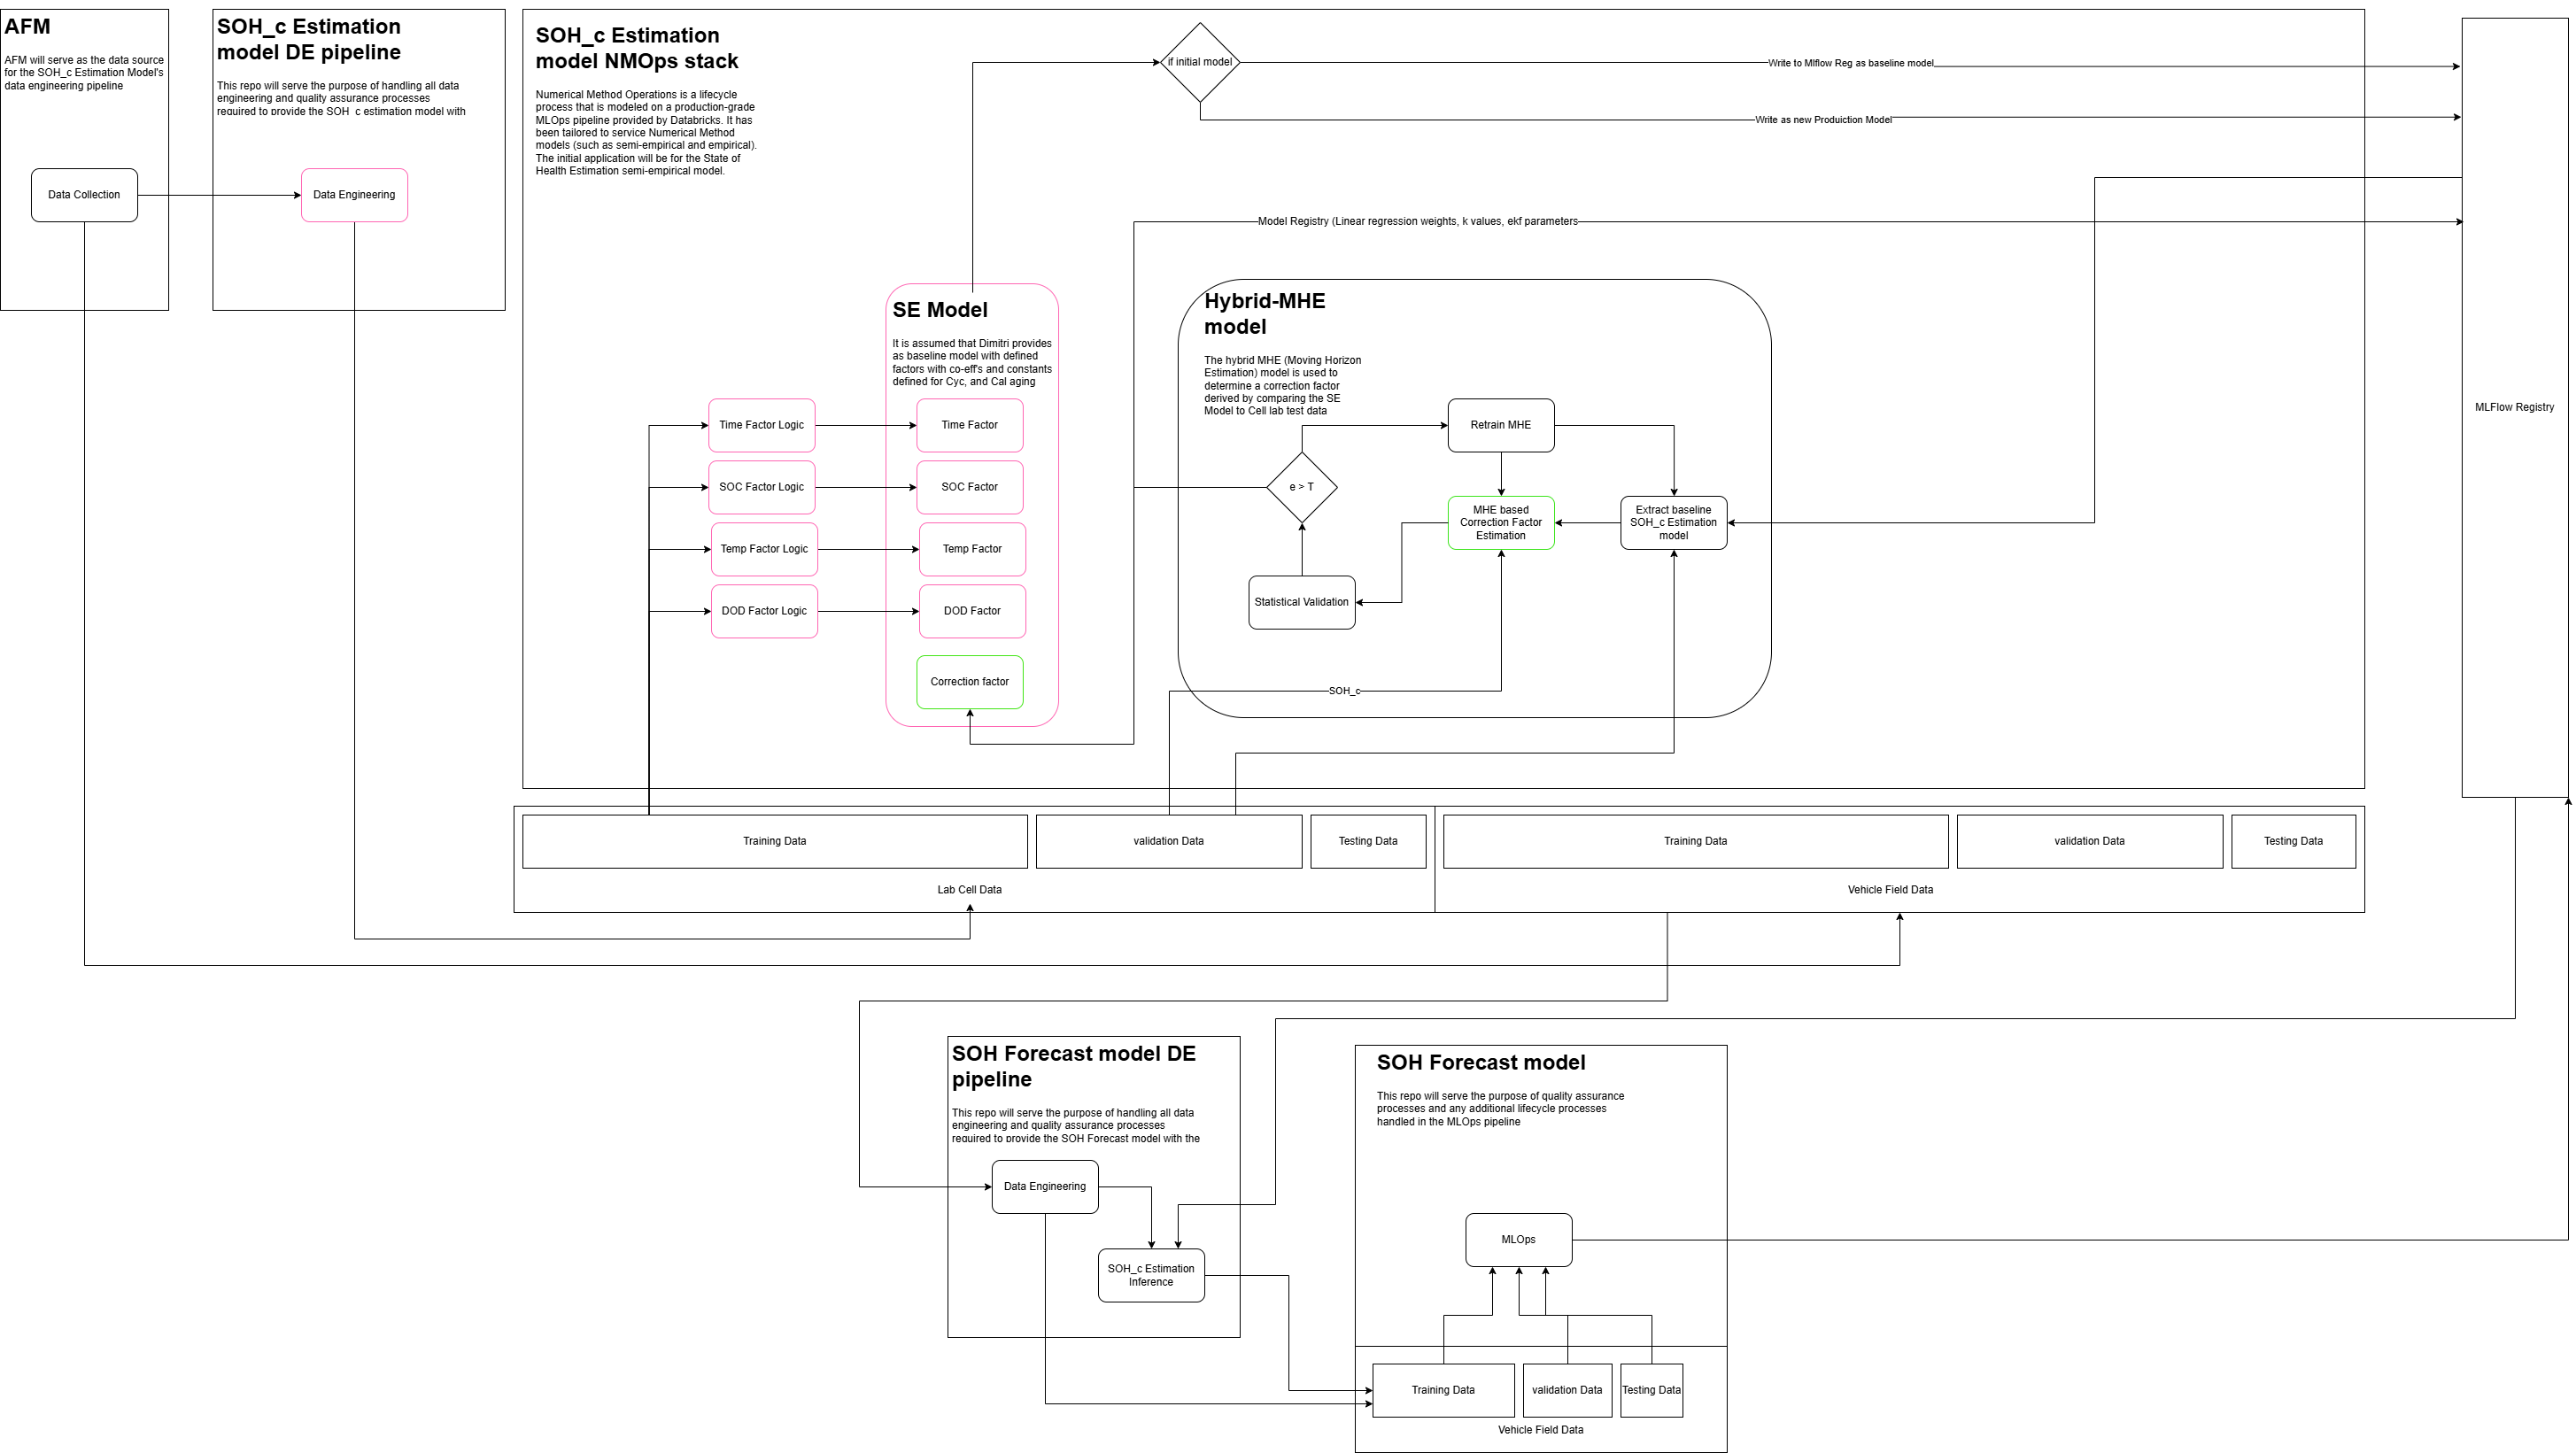
\includegraphics[width=1.0\linewidth]{thesis_template_11-11-17/NMOps-Page-1.drawio.png}
    \caption{NMOps Architecture}
    \label{fig:nmops-architecture}
\end{figure}

\section{Moving Horizon Estimation}
\label{MHE}

\subsection{Overview of Moving Horizon Estimation (MHE)}

Moving Horizon Estimation (MHE) is a deterministic optimization-based approach to dynamic state estimation that relies on a finite history of system measurements. Unlike recursive filters such as the Kalman Filter and its variants, MHE explicitly incorporates system constraints and handles model inaccuracies over a fixed time horizon. This makes it particularly suitable for nonlinear systems and applications requiring bounded estimates.

Consider the general discrete-time nonlinear system:
\begin{align}
x_{k+1} &= f(x_k, u_k) + w_k \\
y_k &= h(x_k) + v_k
\end{align}
where:
\begin{itemize}
    \item $x_k$ denotes the state vector at time step $k$,
    \item $u_k$ is the control input,
    \item $y_k$ represents the output measurement,
    \item $w_k$ and $v_k$ are process and measurement noise, respectively.
\end{itemize}

At each time step $k$, MHE solves an optimization problem over a fixed window of the $N$ most recent measurements to estimate the current state. The cost function minimizes deviations due to noise while incorporating an arrival cost from previous estimates:
\begin{align}
\min_{\{x_i, w_i\}} \quad & \ell(x_{k-N}) + \sum_{i=k-N}^{k-1} \left( \|w_i\|_{Q}^{2} + \|v_i\|_{R}^{2} \right)
\end{align}

subject to the system dynamics and measurement models:
\begin{align}
x_{i+1} &= f(x_i, u_i) + w_i, \quad i = k-N, \ldots, k-1 \\
y_i &= h(x_i) + v_i, \quad i = k-N, \ldots, k
\end{align}

where:
\begin{itemize}
    \item $\ell(x_{k-N})$ is the arrival cost, which penalizes deviation from the prior state estimate,
    \item $Q$ and $R$ are symmetric positive definite matrices weighting the process and measurement residuals,
    \item $\mathcal{X}$ and $\mathcal{W}$ denote the admissible sets for states and disturbances, respectively.
\end{itemize}

This formulation enables MHE to maintain consistency with model constraints and leverage recent measurement data for more robust and accurate state estimates. By optimizing over a horizon rather than a single step, MHE can compensate for delayed information and cope more effectively with modeling errors and transient disturbances.


The outcome of the MHE optimization problem at each time step is an updated state estimate, denoted by $\hat{x}_k$, which reflects the most likely system state given the recent window of inputs and measurements.

Conceptually, MHE is considered the estimation counterpart to Model Predictive Control (MPC). While MPC forecasts optimal control inputs over a future time horizon, MHE operates in the reverse direction—optimizing historical state estimates over a moving window of past data \cite{ZHANG2023108381}. This duality highlights MHE's backward-looking strategy, which enables it to reconstruct states more accurately by leveraging recent information.

One of MHE's key strengths lies in its ability to directly incorporate nonlinear system dynamics and explicit constraints into the estimation problem \cite{KARG2021107266}. For example, physical limitations such as enforcing a state variable to remain within the $[0, 1]$ range can be embedded as hard constraints in the optimization formulation \cite{Rao}. This flexibility gives MHE a distinct advantage over classical filters, such as the EKF, which may generate infeasible or unphysical estimates in constrained scenarios.

Furthermore, in highly nonlinear systems, MHE often delivers superior performance compared to extended Kalman filtering. This is mainly because MHE does not rely on linearization around the current estimate. Instead, it solves a nonlinear optimization problem that considers the entire horizon of measurements, resulting in more globally consistent and accurate state reconstructions \cite{Haseltine}.


While MHE offers significant benefits in flexibility, constraint handling, and nonlinear model accuracy, these advantages come with an inherent computational cost. Each estimation update involves solving an optimization problem, either linear or nonlinear, based on the most recent set of measurements \cite{Kraus}. Although solving such issues in real time may appear demanding, modern numerical solvers have made substantial progress in improving computational efficiency.

Recent implementations have shown that MHE can be executed at update rates in the range of tens of Hertz, even for moderately complex nonlinear systems with up to approximately 100 state variables \cite{Vukov}. These developments make MHE feasible for many embedded and real-time applications, particularly in fields such as battery management, where estimation fidelity is critical and computational hardware continues to evolve.

In summary, MHE delivers a robust and general framework for dynamic state estimation, capable of accommodating nonlinearities and constraints that traditional filtering methods often struggle with. The trade-off is increased computational effort, but this cost is increasingly manageable with current-generation processors and optimized solvers.


\subsection{Formal Definition and Problem Formulation of MHE}

Moving Horizon Estimation (MHE) is typically formulated for discrete-time systems. Continuous-time models, when applicable, are discretized beforehand to fit the MHE framework. The following dynamics and measurement equations describe the system:

\textbf{State Dynamics:}
\begin{equation}
    x_{k+1} = f(x_k, u_k, p) + w_k
\end{equation}

\textbf{Measurement Model:}
\begin{equation}
    y_k = h(x_k, u_k, p) + v_k
\end{equation}

Here:
\begin{itemize}
    \item $x_k \in \mathbb{R}^n$ is the system state at discrete time step $k$,
    \item $u_k$ represents the known control input or excitation,
    \item $y_k$ denotes the measured output,
    \item $f(\cdot)$ is the (possibly nonlinear) state transition function,
    \item $h(\cdot)$ defines the measurement mapping,
    \item $p$ is a vector of known or slowly varying system parameters,
    \item $w_k$ and $v_k$ denote process and measurement noise, respectively.
\end{itemize}

If applicable, physical or operational constraints can be expressed as:
\begin{equation}
    g(x_k, u_k, p) \leq 0
\end{equation}

Let $N$ denote the estimation horizon length. At time $t$, MHE uses the sequence of past measurements $y_{t-N}, \ldots, y_t$ and inputs $u_{t-N}, \ldots, u_{t-1}$ to reconstruct the most probable trajectory of system states:
\[
\{x_{t-N}, x_{t-N+1}, \ldots, x_t\}
\]

This reconstruction is typically formulated as a constrained optimization problem, minimizing a cost function that penalizes deviations from predicted model behavior and sensor observations. The problem is given by:

\begin{align}
    \min_{\{x_k, w_k, v_k\}} \quad & \frac{1}{2} \|x_{t-N} - \hat{x}_{t-N|t-N}\|_P^2 + \frac{1}{2} \sum_{k=t-N}^{t-1} \|w_k\|_{Q^{-1}}^2 + \frac{1}{2} \sum_{k=t-N}^{t} \|v_k\|_{R^{-1}}^2 \label{eq:cost_function} \\
    \text{subject to} \quad & x_{k+1} = f(x_k, u_k, p) + w_k, \quad k = t-N, \ldots, t-1 \\
    & y_k = h(x_k, u_k, p) + v_k, \quad k = t-N, \ldots, t \\
    & g(x_k, u_k, p) \leq 0, \quad k = t-N, \ldots, t
\end{align}

where:
\begin{itemize}
    \item $\hat{x}_{t-N|t-N}$ is the prior state estimate at the start of the horizon,
    \item $P$, $Q$, and $R$ are symmetric positive definite matrices representing weighting on the arrival cost, process noise, and measurement noise, respectively,
    \item The notation $\| \xi \|_M^2 = \xi^\top M \xi$ indicates the squared Mahalanobis norm weighted by $M$.
\end{itemize}

\textbf{Interpretation of Terms:}
\begin{itemize}
    \item The first term penalizes deviation from the prior knowledge of the initial state (arrival cost),
    \item The second term penalizes inconsistency with the model dynamics via process noise,
    \item The third term penalizes mismatch with actual sensor measurements.
\end{itemize}

Often, instead of estimating noise terms explicitly, $w_k$ and $v_k$ are expressed implicitly using the system equations:
\begin{align}
    w_k &= x_{k+1} - f(x_k, u_k, p) \\
    v_k &= y_k - h(x_k, u_k, p)
\end{align}

This substitution reduces the number of optimization variables and simplifies the problem to one of minimizing residual errors in dynamics and measurements.

The constraints must still be satisfied:
\[
x_{k+1} = f(x_k, u_k, p), \quad g(x_k, u_k, p) \leq 0
\]

MHE provides the ability to enforce bounds on states, outputs, or parameters throughout the estimation window—something classical filters like the Kalman filter cannot do explicitly.

At every new time step $t$, the problem is resolved with a shifted window:
\[
\{x_{t-N+1}, \ldots, x_{t+1}\}
\]
incorporating the new measurement $y_{t+1}$ and discarding the oldest data point. This shifting process maintains a fixed optimization window and ensures bounded computational complexity over time.

To express the full problem compactly using bold vectors for trajectories:
\begin{align}
    \min_{\bm{x}, \bm{w}, \bm{v}} \quad & \frac{1}{2} \|x_{t-N} - \hat{x}_{t-N|t-N}\|_P^2 + \frac{1}{2} \sum_{k=t-N}^{t-1} \|w_k\|_{Q^{-1}}^2 + \frac{1}{2} \sum_{k=t-N}^{t} \|v_k\|_{R^{-1}}^2 \\
    \text{subject to} \quad & x_{k+1} = f(x_k, u_k, p) + w_k \\
    & y_k = h(x_k, u_k, p) + v_k, \quad k = t-N, \ldots, t
\end{align}

Tuning the weighting matrices $P$, $Q$, and $R$ is essential. The arrival cost weight $P$ in particular plays a significant role in determining estimator stability and how much historical confidence is placed on the prior state.


\subsection{Assumptions and Theoretical Properties of MHE}

For Moving Horizon Estimation (MHE) to yield accurate and reliable results, certain theoretical conditions related to observability and stability must be satisfied. Specifically, the underlying system must be sufficiently observable over the moving window, and the estimation scheme must ensure bounded error as new measurements are incorporated \cite{ALESSANDRI2025112187}.

A key assumption is that the system exhibits \textit{observability}, that is, the sequence of measured outputs over the horizon must contain enough information to distinguish between different internal states. A stronger condition known as \textit{uniform observability} is required in many cases. This ensures that two distinct state trajectories result in sufficiently different output sequences over the window, as formalized through bounds involving class $\mathcal{K}$ functions \cite{Flayac_2021}.

If the horizon length $N$ is chosen to be at least as large as the system’s observability index, assuming no model mismatch or measurement noise, it is theoretically possible to reconstruct the exact state. In realistic scenarios with process and sensor noise, uniform observability guarantees that the estimation error remains bounded rather than diverging over time \cite{5718126}.

Another essential component of the MHE formulation is the \textit{arrival cost}, sometimes referred to as the prior term. Since MHE discards older measurements outside the current estimation window, the arrival cost serves to incorporate prior information and prevent estimation drift due to unmodeled past disturbances \cite{deniz2019robuststabilitymovinghorizon}. This term acts as a compact representation of all earlier information not captured within the current horizon.

If appropriately designed, the arrival cost enhances the estimator’s stability. It is often constructed to approximate either the optimal cost-to-go from a full-information estimator or the state covariance, as would be computed by a dual Kalman filter or a Riccati-based method. Theoretical guarantees show that, under conditions such as uniform observability and a properly defined arrival penalty, the estimation error of the MHE scheme remains asymptotically stable.

Two key performance guarantees that can be established under these conditions are:
\begin{itemize}
    \item Convergence of the estimated state to the true state in the ideal (noise-free) case,
    \item Bounded estimation error in the presence of bounded process and measurement noise.
\end{itemize}

In the presence of modeling errors or external disturbances, MHE can exhibit \textit{Input-to-State Stability} (ISS), where the magnitude of estimation error is bounded proportionally to the disturbance magnitude \cite{Ji}. This ensures robustness against imperfections in both the model and sensor data.

Stability analysis for MHE often relies on Lyapunov-based arguments or draws from the properties of full-information estimators. By using a sufficiently large horizon length and a well-tuned arrival cost, it is possible to bound the estimation error over time \cite{Schiller_2023}.

Even in cases where the system is not completely observable at all times, a relaxed condition known as \textit{detectability} may be sufficient. If the unobservable modes are asymptotically stable, the estimator can still maintain bounded error \cite{Schiller_2024}.

Additionally, MHE inherently provides robustness to outliers and transient sensor faults due to its batch optimization nature. The aggregated cost across multiple time steps prevents single erroneous measurements from significantly influencing the state estimate \cite{Schiller_2023}. To further improve robustness, non-quadratic penalties such as the Huber loss can be employed in the cost function, reducing sensitivity to outliers and model mismatch.

\textbf{In summary}, when system observability and model fidelity conditions are satisfied, MHE possesses strong theoretical guarantees. Specifically, it can:
\begin{itemize}
    \item Converge to the correct state trajectory as more data is accumulated,
    \item Maintain bounded error even in noisy or uncertain environments.
\end{itemize}

Achieving these properties in practical implementations requires careful design choices, especially regarding:
\begin{itemize}
    \item The estimation horizon length $N$,
    \item The structure and weight of the arrival cost term.
\end{itemize}

A horizon that is too short may behave similarly to a high-gain filter, making the estimator sensitive to noise. Conversely, increasing $N$ improves estimation accuracy at the expense of computational complexity. Hence, selecting $N$ involves balancing estimation quality against available processing resources.


\subsection{References and Example Implementations}

There is a growing body of literature and practical experimentation supporting the use of MHE in battery state estimation applications. The techniques outlined in previous sections have been validated through both academic research and early-stage industrial deployments:

\begin{itemize}
    \item \textbf{Joint State and Parameter Estimation:}  
    Several recent works extend MHE to jointly estimate system states and slowly varying parameters, such as battery capacity. In these formulations, capacity is modeled as an additional state that evolves gradually. For example, \cite{Yongzhe} presents an MHE-based method where regularization terms—functionally similar to arrival costs- are added to penalize abrupt changes in capacity unless strongly supported by the data. This enables real-time State of Health (SOH) tracking through consistent, smooth estimation of capacity fade during charge–discharge cycles.

    \item \textbf{Real-Time MHE for Embedded BMS:}  
    To enable deployment in resource-constrained embedded battery management systems (BMS), researchers have proposed computationally efficient variants of MHE. For instance, the "fast embedded MHE" method reduces complexity by using shortened horizons and partial state updates, making it suitable for low-power microcontrollers \cite{wan2024towards}. Other studies introduce multi-rate MHE architectures, exploiting that current can often be measured at higher frequencies than voltage. In such schemes, fast current-based updates are complemented by slower but more accurate voltage-based corrections, balancing accuracy and runtime efficiency.
\end{itemize}

The methods discussed here are presented generally, focusing on the underlying mathematical principles and estimation framework. These formulations are designed to be independent of specific datasets or implementation platforms. The next chapter details their practical application, including dataset characteristics, parameter selection, model tuning, and evaluation on real battery systems.


\section{Adaptive Multi-Horizon Correction Algorithm}
\label{algo}
The Adaptive Multi-Horizon Correction Algorithm is illustrated in \ref{alg:algorithm}. We will go through the steps and mathematical formulations that leverage adaptive correction factors, weighted optimization, and sequential smoothing to track SOH dynamics over battery life cycles robustly. 

\subsection{Methodology}
The Adaptive Multi-Horizon Correction Algorithm follows a sequential process consisting of:
\begin{itemize}
    \item Battery Data Processing.
    \item Adaptive window size estimation.
    \item MHE Optimization using Bayesian Search (Optuna).
    \item Weighted Averaging and stacking with Linear Regression.
    \item EKF-based smoothing and Residual Correction.
    \item Error Metrics Computation.
\end{itemize}

\subsubsection{Inputs and Outputs}
\begin{itemize}
    \item \textbf{Inputs:} \begin{itemize}
        \item \textbf{dataset\_folder:} Directory containing battery datasets.
        \item \textbf{battery\_params:} Dictionary with battery specifications.
        \item \textbf{n\_trials\_mhe:} Number of Optimization trials for MHE.
        \item \textbf{n\_trials\_ekf:} Number of Optimization trials for EKF.
    \end{itemize}
    \item \textbf{Outputs:} \begin{itemize}
        \item \textbf{all\_results:} Dictionary storing optional parameters, SOH predictions, and error metrics for each battery.
    \end{itemize}
\end{itemize}

\subsubsection{Battery Preprocessing}
Each battery dataset is first processed to extract:
\begin{itemize}
    \item \textbf{Final\_cyclic\_aging:} SOH estimate from the Semi-Empirical model.
    \item \textbf{Ground\_truth\_soh:} SOH from the test bench data.
\end{itemize}
Final cyclic aging is rescaled to match the mean of the ground truth:
\begin{equation}
    \text{Final\_cyclic\_aging\_scaled} = \text{Final\_cyclic\_aging} \times \frac{\mu_{\text{fa}}}{\mu_{\text{gt}}}
\end{equation}
Where:
\begin{itemize}
    \item $\mu_{\text{gt}}$ is the mean of the ground truth sequence,
    \item $\mu_{\text{fa}}$ is the mean of the final cyclic aging sequence.
\end{itemize}

\subsubsection{Adaptive Window Size Computation}
To handle varying degradation rates, window sizes are adapted based on SOH changes:
\begin{enumerate}
    \item Computer first differences: \begin{equation}
    \Delta \text{SOH}_i = \left| \text{SOH}_{i+1} - \text{SOH}_i \right|\end{equation}
    \item Define a threshold $\tau$ as the 75th percentile of the set of first differences $\Delta \text{SOH}$.
    \item Assign window sizes according to:
\begin{equation}
\text{window\_size}_i = 
\begin{cases}
3, & \text{if } \Delta \text{SOH}_i > \tau \\
10, & \text{otherwise}
\end{cases}
\end{equation}
\end{enumerate}

\subsubsection{Moving Horizon Estimation (MHE)}
For each unique window size, the MHE problem is formulated as a minimization of a hybrid objective function involving:
\begin{itemize}
    \item \textbf{Huber Loss} for robust error handling: \begin{equation}
L_\delta(r) = 
\begin{cases}
\frac{1}{2} r^2, & \text{if } |r| \leq \delta \\
\delta (|r| - \frac{1}{2} \delta), & \text{otherwise}
\end{cases}
\end{equation}
where:
\begin{itemize}
    \item \( r \) is the residual between the corrected State of Health (SOH) and the ground truth,
    \item \( \delta = 1.0 \) is the threshold parameter.
\end{itemize}
\item Define the penalty term \( k_{\text{penalty}} \) as:
\begin{equation}
k_{\text{penalty}} = 
\begin{cases}
1000 \times \left( |k - k_{\text{prev}}| - 0.1 \right), & \text{if } |k - k_{\text{prev}}| > 0.1 \\
0, & \text{otherwise}
\end{cases}
\end{equation}
Where:
\begin{itemize}
    \item \( k \) is the current correction factor,
    \item \( k_{\text{prev}} \) is the previous correction factor.
\end{itemize}
\item Define the L2 regularization penalty as:
\begin{equation}
L2_{\text{penalty}} = 0.01 \times k^2
\end{equation}
where:
\begin{itemize}
    \item \( k \) is the correction factor or model parameter being regularized.
\end{itemize}
\item Define the penalty based on the Mean Squared Error (MSE) as:
\begin{equation}
\text{penalty} = 
\begin{cases}
1000 \times | \text{MSE} - 17 |, & \text{if } \text{MSE} < 9 \text{ or } \text{MSE} > 25 \\
0, & \text{otherwise}
\end{cases}
\end{equation}
Where:
\begin{itemize}
    \item MSE is the Mean Squared Error between predicted and ground truth values.
\end{itemize}
\end{itemize}
Thus, the Moving Horizon Estimation (MHE) optimization objective is defined as:
\begin{equation}
\text{Objective} = \text{Huber Loss} + k_{\text{penalty}} + L2_{\text{penalty}} + \text{penalty}
\end{equation}
Where:
\begin{itemize}
    \item \textbf{Huber Loss} penalizes residual errors between the corrected SOH and ground truth,
    \item \( k_{\text{penalty}} \) penalizes large deviations in the correction factor \(k\),
    \item \( L2_{\text{penalty}} \) provides regularization to keep \(k\) small,
    \item \textbf{penalty} enforces the MSE to remain within the desired range \([9, 25]\).
\end{itemize}

Bayesian optimization, implemented via the Optuna framework \cite{akiba2019optunanextgenerationhyperparameteroptimization}, is employed to find the global optimum.

\subsubsection{Weighted Averaging of MHE Solutions}
After solving individual MHE problems, a weighted aggregation is performed to compute the corrected SOH as:
\begin{equation}
\text{Corrected\_SOH} = \sum_i \left( \frac{w_i}{\sum_j w_j} \times k_i \times \text{Final\_cyclic\_aging\_scaled} \right)
\end{equation}
Where:
\begin{itemize}
    \item \( w_i = \frac{1}{\text{loss}_i} \) is the weight assigned to the \(i\)-th MHE solution, inversely proportional to its associated loss,
    \item \( k_i \) is the correction factor from the \(i\)-th MHE,
    \item \text{Final\_cyclic\_aging\_scaled} is the scaled cyclic aging sequence.
\end{itemize}

\subsubsection{Stacking Model: Linear Regression}
A simple stacked regression model is trained as:
\begin{equation}
\text{Stacked\_SOH} =\\ \alpha \times \text{Final\_cyclic\_aging\_scaled} + \beta \times \text{Local\_Corrected\_SOH} + \gamma
\end{equation}
where:
\begin{itemize}
    \item \( \alpha, \beta, \gamma \) are coefficients learned by minimizing the least squares error.
\end{itemize}

\subsubsection{EKF Smoothing}
Using the following equations, an Extended Kalman Filter (EKF) is applied to reduce sequential noise.

State Prediction:

\begin{align}
x_{k|k-1} &= x_{k-1} + \text{trend\_rate} \\
P_{k|k-1} &= P_{k-1} + Q
\end{align}

Measurement Update:

\begin{align}
K_k &= \frac{P_{k|k-1}}{P_{k|k-1} + R} \\
x_k &= x_{k|k-1} + K_k (z_k - x_{k|k-1}) \\
P_k &= (1 - K_k) P_{k|k-1}
\end{align}

Where:
\begin{itemize}
    \item \( Q \) and \( R \) represent the process and measurement noise covariances, respectively,
    \item \( \text{trend\_rate} \) is a drift term accounting for expected gradual changes in the state.
\end{itemize}

Hyperparameter Optimization:

The hyperparameters \( Q \), \( R \), and \( \text{trend\_rate} \) are optimized via Bayesian optimization using the Optuna framework \cite{akiba2019optunanextgenerationhyperparameteroptimization}, to minimize the post-smoothing Huber loss.

\subsubsection{Error Metrics}
The final evaluation metrics include:

Mean Squared Error (MSE):

\begin{equation}
\text{MSE} = \frac{1}{N} \sum_{i=1}^{N} (y_i - \hat{y}_i)^2
\end{equation}

Root Mean Squared Error (RMSE):

\begin{equation}
\text{RMSE} = \sqrt{\text{MSE}}
\end{equation}

Both metrics are computed against the ground truth and the scaled cyclic aging baselines.


\begin{algorithm}
\caption{Battery SOH Estimation with MHE, Stacking, and EKF}
\label{alg:algorithm}
\begin{algorithmic}[1]
\ENSURE all\_results (dictionary)

\STATE Load battery parameters from \texttt{battery\_params.json} into \texttt{params}
\STATE Initialize \texttt{all\_results = \{\}}

\FOR{each \texttt{battery\_name} in \texttt{params}}
    \STATE \texttt{macro\_df = process\_battery(battery\_name, dataset\_folder)}
    \STATE Scale \texttt{Final\_cyclic\_aging}:
    \STATE \hspace{0.5cm} \texttt{scaling\_factor = mean(ground\\\_truth\_soh) / mean(Final\_cyclic\_aging)}
    \STATE \hspace{0.5cm} \texttt{Final\_cyclic\_aging\_scaled = Final\_cyclic\_aging} $\times$ \texttt{scaling\_factor}

    \STATE Compute adaptive \texttt{window\_sizes} based on 75th percentile of $\Delta$SOH.

    \STATE Initialize \texttt{mhe\_results = [ ]}, \texttt{prev\_k = None}

    \FOR{each unique \texttt{window\_size} in \texttt{window\_sizes}}
        \STATE Initialize Optuna study (TPE Sampler, startup trials=20)
        \FOR{each trial (n\_trials\_mhe // number of unique window sizes)}
            \STATE Suggest \texttt{window\_size} and \texttt{global\_k}
            \STATE Compute objective combining Huber Loss, k\_penalty, L2\_penalty, and MSE penalties
        \ENDFOR
        \STATE Store best (\texttt{window\_size}, \texttt{global\_k}, \texttt{loss}) in \texttt{mhe\_results}
        \STATE Update \texttt{prev\_k}
    \ENDFOR

    \STATE Perform weighted averaging of MHE results to compute \texttt{Local\_Corrected\_SOH}

    \STATE Apply stacking (Linear Regression) to predict \texttt{Stacked\_SOH} from \texttt{Final\_cyclic\_aging\_scaled} and \texttt{Local\_Corrected\_SOH}

    \STATE Apply EKF smoothing:
    \STATE \hspace{0.5cm} Initialize Optuna study (startup trials=10)
    \STATE \hspace{0.5cm} Optimize (Q, R, trend\_rate)
    \STATE \hspace{0.5cm} Run EKF to compute \texttt{Smoothed\_SOH}

    \STATE Compute error metrics: MSE, RMSE against ground truth and final cyclic aging.

    \STATE Save \texttt{macro\_df} to file and update \texttt{all\_results[battery\_name]} with results.

    \STATE Print optimization values and plot SOH curves.
\ENDFOR

\RETURN \texttt{all\_results}

\end{algorithmic}
\end{algorithm}

\subsection{Example}
This section illustrates the application of optimized correction factors ($k$ values) to battery degradation data. Using a simple 10-cycle example, we demonstrate how correction factors, optimized by Moving Horizon Estimation (MHE), are blended through weighted averaging to enhance State of Health (SOH) prediction.

\textbf{Problem Setup}

We consider a battery named \texttt{B0005} with data for 10 cycles:

\begin{itemize}
    \item \textbf{Cycle indices}: $[0, 1, 2, 3, 4, 5, 6, 7, 8, 9]$
    \item \textbf{Final\_cyclic\_aging\_scaled} (\%): $[80, 79, 78, 77, 76, 75, 74, 73, 72, 71]$
    \item \textbf{Ground truth SOH} (\%): $[81, 80, 79, 78, 77, 76, 75, 74, 73, 72]$
\end{itemize}

The goal is to correct the \texttt{Final\_cyclic\_aging\_scaled} series so it closely matches the ground truth SOH.

Two window sizes were selected based on SOH change dynamics:
\begin{itemize}
    \item Window size 3 (sensitive to short-term changes)
    \item Window size 10 (captures global trends)
\end{itemize}

The optimized correction factors obtained via MHE are:
\[
k_1 = 1.0125 \quad (\text{for window size 3}), \qquad k_2 = 1.0140 \quad (\text{for window size 10})
\]
The associated optimization losses are:
\[
\text{Loss}_1 = 10, \quad \text{Loss}_2 = 12
\]

\textbf{Correction Process}

\textbf{Applying $k_1$ for Window Size 3}

The 10 cycles are partitioned into windows of size 3:

\[
[0,1,2],\quad [3,4,5],\quad [6,7,8],\quad [9]
\]

Applying $k_1$ to each chunk:

\begin{align*}
\text{Chunk [0-2]} &: [80, 79, 78] \times 1.0125 = [81.000, 79.9875, 78.975]\\
\text{Chunk [3-5]} &: [77, 76, 75] \times 1.0125 = [77.9625, 76.9500, 75.9375]\\
\text{Chunk [6-8]} &: [74, 73, 72] \times 1.0125 = [74.925, 73.9125, 72.900]\\
\text{Chunk [9]}   &: [71] \times 1.0125 = [71.8875]
\end{align*}

Thus, the whole corrected series for window size 3 is:

\[
\text{SOH}_3 = [81.000, 79.9875, 78.975, 77.9625, 76.950, 75.9375, 74.925, 73.9125, 72.900, 71.8875]
\]

\textbf{Applying $k_2$ for Window Size 10}

For window size 10, the entire dataset is treated as a single window:

\[
[0,1,2,3,4,5,6,7,8,9]
\]

Applying $k_2$:

\begin{align*}
\text{SOH}_{10} = &[80 \times 1.0140, 79 \times 1.0140, 78 \times 1.0140, 77 \times 1.0140,\\
&76 \times 1.0140, 75 \times 1.0140, 74 \times 1.0140, 73 \times 1.0140, 72 \times 1.0140, 71 \times 1.0140] \\
= &[81.120, 80.106, 79.092, 78.078, 77.064, 76.050, 75.036, 74.022, 73.008, 71.994]
\end{align*}

\textbf{Computing Weights for Blending}

The weights are computed as the inverse of the optimization losses:

\[
\text{Weight}_1 = \frac{1}{10} = 0.1, \quad \text{Weight}_2 = \frac{1}{12} \approx 0.08333
\]
Total weight:
\[
\text{Total Weight} = 0.1 + 0.08333 = 0.18333
\]
Normalized weights:
\[
\text{Normalized Weight}_1 = \frac{0.1}{0.18333} \approx 0.54545, \quad \text{Normalized Weight}_2 = \frac{0.08333}{0.18333} \approx 0.45455
\]

\textbf{Blending the Corrected SOHs}

The final corrected SOH at each cycle is computed by weighted averaging:

\[
\text{Final SOH}_i = (0.54545 \times \text{SOH}_3[i]) + (0.45455 \times \text{SOH}_{10}[i])
\]

Example calculations:

\begin{align*}
\text{Cycle 0}: \quad &81.0545 = (0.54545 \times 81.000) + (0.45455 \times 81.120)\\
\text{Cycle 1}: \quad &80.0402 = (0.54545 \times 79.9875) + (0.45455 \times 80.106)\\
\text{Cycle 2}: \quad &79.0260 = (0.54545 \times 78.975) + (0.45455 \times 79.092)\\
\end{align*}

Following the same blending process for all cycles yields:

\[
\text{Local\_Corrected\_SOH} \approx [81.0545, 80.0402, 79.0260, 77.9977, 76.9834,~75.9692,~74.9550,....]
\]

This example illustrates how multiple MHE-optimized correction factors ($k_1$ and $k_2$) are applied to different window sizes and blended to produce a robust SOH trajectory. The final SOH curve benefits from local sensitivity and global consistency by giving more weight to correction factors with lower losses.


%%%%%%%%%%%%%%%%%%%%%%%%%%%%%%%%%%%%%%%%%%%%%%%%%%%%%%%%%%%%
\chapter{Experimental Evaluation}
\label{chap:eval}
In this chapter, we outline the implementation of our NMOps architecture, as described in \ref{fig:nmops-architecture}, incorporating best practices from MLOps frameworks, as summarized in \ref{MLOPS}, and the algorithm presented in section \ref{alg:algorithm}.

Some of the process, usage, and requirements of the NMOps are given below:
\begin{enumerate}
    \item \textbf{Data pipeline:}\begin{itemize}
        \item \textbf{Ingestion:} Connect to Azure Data Lake to pull battery telemetry (cycles, voltage, current, temperature) in batch mode.
        \item \textbf{Preprocessing:} Automate scaling and window size computation using a workflow orchestrator. Store pre-computed mean for efficiency. Validate data quality (no missing values, numerical consistency).
        \item \textbf{Scheduling:} Run daily or event-triggered preprocessing jobs to handle new data.
        \item \textbf{Tools:} Kuberflow, Pandas/Spark for transformations.
    \end{itemize}
    \item \textbf{Model Training Pipeline:} \begin{itemize}
        \item \textbf{Training:} Encapsulate MHE, stacking, and EKF optimization in a training pipeline. Log parameters ($k_1$, $k_2$, regression weights, Q, R, trend\_rate) and metrics (MSE, RMSE) using MLflow. Support parallel training with Dask or Spark.
        \item \textbf{Hyperparamete Tuning:} Automate Optuna runs for MHE and EKF, storing best paramters in a MLflow model registry.
        \item \textbf{Frequency:} Train weekly or when data drift is detected. 
        \item \textbf{Tools:} MLflow for logging, SageMaker for cloud training, Kuberflow for orchestration.
    \end{itemize}
    \item \textbf{Model Deployment}: \begin{itemize}
        \item \textbf{Serving:} Deploy a REST API or serverless function to correct SOH in real-time.
        \item \textbf{Batch Inference:} Support batch processing for historical data using scheduled jobs.
        \item \textbf{Model Registry:} Store trained models (linear regression weights, $k$ values, EKF parameters) with versioning.
        \item \textbf{Scaling:} Auto-scaling to handle variable loads.
        \item \textbf{Tools:} FastAPI for API, Docker for containerization, Kubernetes for orchestration.
    \end{itemize}
    \item \textbf{Monitoring and Maintenance:} \begin{itemize}
        \item \textbf{Performance Monitoring:} Track RMSE\_ground\_truth and \\ RMSE\_final\_cyclic daily using a dashboard. Alert if RMSE>5\% (indicating correction degradation).
        \item \textbf{Data Drift:} Monitor Final\_cyclic\_againg\_scaled distribution for shifts (e.g., mean change > 10\%).
        \item \textbf{Model Drift:} Compare predictions against new ground truth data to detect performance drops.
        \item \textbf{Logging:} Log API requests, prediction errors, and retraining events to a centralized system.
        \item \textbf{Tools:} Grafana for dashboards, Prometheus for alerts.
    \end{itemize}
    \item \textbf{CI/CD and Retraining:}\begin{itemize}
        \item \textbf{Continuous Integration:} Automate testing of code updates using GitHub Actions.
        \item \textbf{Continuous Delivery:} Deploy updated models to production endpoints when retrained with rollback support via model registry.
        \item \textbf{Retraining Triggers:} Retrain on new data weekly, when RMSE>5\%, or when drift is detected.
        \item \textbf{Tools:} GitHub Actions for CI, Jenkins for CD, MLflow for model versioning.
    \end{itemize}
    \item \textbf{Infrastructure:} \begin{itemize}
        \item \textbf{Cloud:} Deploy on Azure with managed services.
        \item \textbf{Containerization:} Package algorithm in Docker containers for consistent deployment.
        \item \textbf{Orchestration:} Use Kubernetes for scaling and managing API services.
    \end{itemize}
    \item \textbf{Operational Requirements:}\begin{itemize}
        \item \textbf{Deployment:} Support batch processing for historical data and real-time API for live SOH correction. Ensure 99.9\% uptime for production APIs, with auto-scaling in cloud environments.
        \item \textbf{Monitoring:} Monitor RMSE\_ground\_truth daily, alerting if >5\%. Track data drift in the Final cyclic aging scaled. Log model performance and retraining events in the dashboard.
        \item \textbf{Maintenance:} Schedule weekly retraining or when drift is detected. Update the correction logic based on feedback. Maintain documentation and version control.
    \end{itemize}
    \item \textbf{Constraints and Assumptions:} \begin{itemize}
        \item \textbf{Constraints:} \begin{itemize}
            \item Limited to numerical cycle data with no missing values.
            \item Sequential processing limits scalability; large-scale use requires parallelization.
            \item Optuna optimization is CPU-bound, slowing down large datasets.
        \end{itemize}
        \item \textbf{Assumptions:} \begin{itemize}
            \item Final cycling aging is a semi-empirical SOH estimate, reasonably accurate.
            \item Ground truth SOH is available for training and validation.
            \item Battery data is clean and representative of EV/storage use cases.
            \item Cloud resources are available for scaling.
        \end{itemize}
    \end{itemize}
\end{enumerate}

The battery SOH estimation project requires robust requirements to deliver accurate, scalable, and maintainable predictions. Correcting semi-empirical SOH estimates using MHE, stacking, and EKF supports critical applications, such as electric vehicle (EV) fleet management. Integration into an MLOps architecture—via automated data pipelines, training, deployment, monitoring, and continuous integration/continuous deployment (CI/CD)—ensures continuous improvement and reliability in production. With parallelization, distributed computing, and MLOps tools, it scales to large datasets and fits seamlessly into modern ML workflows.

\subsection{Dataset}

This study utilizes the NASA Lithium-Ion Battery Dataset, made publicly available by the Prognostics Center of Excellence (PCoE) at NASA Ames Research Center. The dataset has become a benchmark for researching battery health diagnostics, performance forecasting, and remaining useful life (RUL) prediction. It is widely adopted in both academic and industrial settings.

The dataset contains time-series data collected from commercial lithium-ion cells operated under controlled test conditions until they reached their end-of-life, which is defined as the point where battery capacity falls below 70\% of the rated nominal value. Each battery was subjected to repeated charge–discharge cycles, during which parameters such as voltage, current, temperature, and capacity were continuously recorded.

The batteries were tested under various cycling protocols to simulate real-world degradation behavior, including different charge/discharge currents and thermal environments. This results in diverse degradation trajectories across the dataset, which helps in training and validating robust predictive models.

The dataset is particularly valuable due to its incorporation of practical challenges such as sensor noise, non-linear aging behavior, and inter-cycle variability. These characteristics make it suitable not only for capacity forecasting but also for tasks like fault detection, anomaly identification, and model generalization. As such, the NASA dataset provides a realistic and comprehensive testbed for developing and evaluating algorithms for battery prognostics and health management.


\subsubsection{Dataset Structure}
Figure \ref{fig:data-structure} illustrates the structure of the NASA dataset used. The data is grouped by battery. Each battery (e.g., B005) has its dataset. For each battery, the entire life of the battery is divided into individual charge-discharge cycles. Each cycle contains the cycle number, charge data, discharge data, capacity measurement, and time stamps. The recorded data included Voltage (V), Current (A), Temperature (\degree C), and Capacity (Ah). Batteries were considered to have failed when their capacity dropped to 70\% of their nominal capacity (2.0 Ah).

\subsubsection{Testing Conditions}
The batteries were cycled under different operating conditions, including varying charge/discharge rates (C-rates), temperature variations, and different state-of-charge windows (e.g., charging between 4.2 V and 2.5 V)

\begin{figure}
    \centering
    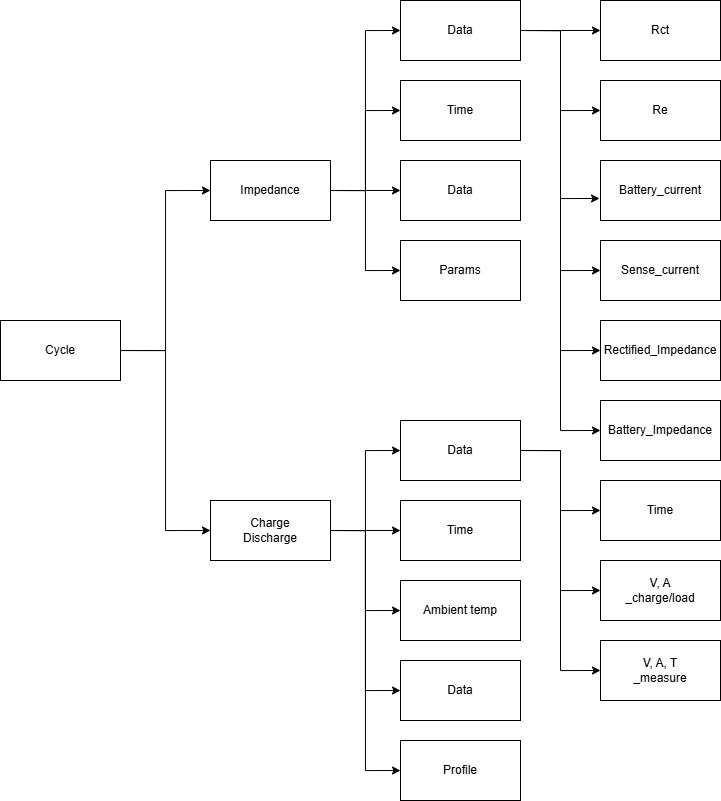
\includegraphics[width=0.5\linewidth]{thesis_template_11-11-17/data_structure.drawio (1).png}
    \caption{Structure of the NASA dataset}
    \label{fig:data-structure}
\end{figure}

\subsubsection{Datasets Included}
The dataset is grouped into two major sets:
\begin{itemize}
    \item \textbf{Battery Data Set 1:} Batteries were charged and discharged under a regime to accelerate aging.
    \item \textbf{Battery Data Set 2:} Different operational regimes were applied across batteries, some subjected to constant loads, others to variable loads.
\end{itemize}

\subsubsection{Data Format}
Stored in .mat (MATLAB format) files, but converted to CSV for convenience. Each battery has a file containing structured data across hundreds or thousands of cycles.

\subsubsection{Challenges in the Dataset}
\begin{itemize}
    \item \textbf{Noise:} Real-world noise is present in the measurements, making it realistic but challenging.
    \item \textbf{Cycle Variability:} Cycle-to-cycle variations exist, requiring careful preprocessing.
    \item \textbf{Non-linear degradation:} Battery health does not degrade linearly over time; sudden drops may occur.
\end{itemize}

\subsection{Exploratory Data Analysis}
In this section, we aim to gain some insights into the data that will be used to correct SOH estimation using the NMOps Architecture. We will conduct a deep dive into data quality analysis, including missing values, trend analysis (such as capacity degradation, voltage behavior, and Temperature trends), and a statistical summary of the battery dataset, which is crucial for further implementation and experiments. 

Our EDA will focus on key variables (e.g., capacity, voltage, current, temperature) to understand battery behavior and degradation patterns.

\textbf{EDA Objectives}
\begin{itemize}
    \item \textbf{Understand Data Structure:} Explore the .mat file format and extract relevant measurements.
    \item \textbf{Summarize Key Variables:} Analyze capacity, voltage, current, and temperature distributions.
    \item \textbf{Visualize Degradation Trends:} Plot SOH and other metrics over cycles to observe aging.
    \item \textbf{Identify Patterns and Anomalies:} Detect fluctuations, outliers, or test condition effects.
    \item \textbf{Prepare for Modeling:} Highlight insights for SOH prediction or RUL estimation.
\end{itemize}

Table \ref{tab:eda1} from the exploratory data analysis (EDA) code for the NASA Battery Dataset, specifically for battery B0005, provides valuable insights into the structure and characteristics of the discharge cycle data. Below, I will analyze the output, explaining its meaning, implications for the dataset, and how it informs further analysis or modeling of battery State of Health (SOH).

\begin{table}[h!]
\centering
\begin{tabular}{@{}clcc@{}}
\toprule
\# & \textbf{Column} & \textbf{Non-Null Count} & \textbf{Dtype} \\ 
\midrule
0 & cycle                 & 168 & int64    \\
1 & ambient\_temperature   & 168 & float64  \\
2 & capacity              & 168 & float64  \\
3 & voltage\_measured      & 168 & object   \\
4 & current\_measured      & 168 & object   \\
5 & temperature\_measured  & 168 & object   \\
6 & time                  & 168 & object   \\
\bottomrule
\end{tabular}
\caption{Summary of the dataset columns, non-null counts, and data types.}
\label{tab:eda1}
\end{table}

\begin{itemize}
    \item \textbf{Shape:} The DataFrame has 168 rows, corresponding to 168 discharge cycles for battery B0005. Each row represents one discharge cycle.
    \item \textbf{Columns:} There are 7 columns: \begin{itemize}
        \item cycle: Cycle number (int64, 1 to 168).
        \item ambient\_temperature: Ambient temperature during testing (float64).
        \item capacity: Measured battery capacity in ampere-hours (Ah, float64).
        \item voltage\_measured, current\_measured, temperature\_measured, time: Time-series measurements stored as objects (likely NumPy arrays or lists).
    \end{itemize}
    \item \textbf{Non-Null Counts:} All 168 entries are non-null for all columns, indicating no missing data in the extracted dataset.
    \item \textbf{Data Types:} cycle, ambient\_temperature, and capacity are numeric (int64 or float64), suitable for analysis. voltage\_measured, current\_measured, temperature\_measured, and time are object types, suggesting they are arrays/lists of measurements per cycle, which require further processing for scalar analysis.
\end{itemize}

\textbf{Analysis:}
\begin{itemize}
    \item The dataset is complete with no missing values, which is ideal for analysis.
    \item The object type for time-series data (e.g., voltage\_measured) indicates that each entry is an array of measurements taken during the discharge cycle. To analyze these (e.g., mean voltage), we must extract scalar features (e.g., average, min, max) or process them separately.
    \item The numeric columns (capacity, SOH) are ready for statistical analysis and visualization.
\end{itemize}

\begin{table}[h!]
\centering
\begin{tabular}{cc}
\toprule
\textbf{Index} & \textbf{Capacity (Ah)} \\
\midrule
0 & 1.856487 \\
1 & 1.846327 \\
2 & 1.835349 \\
3 & 1.835263 \\
4 & 1.834646 \\
5 & 1.835662 \\
6 & 1.835146 \\
7 & 1.825757 \\
8 & 1.824774 \\
9 & 1.824613 \\
\bottomrule
\end{tabular}
\caption{Sample values from the \texttt{capacity} column.}
\label{tab:capacity_sample}
\end{table}


Table \ref{tab:capacity_sample} is the capacity values (in Ah) for the first 10 discharge cycles of B0005.
\begin{itemize} 
    \item Initial capacity is high (~1.856 Ah in cycle 1), close to the nominal capacity of 2 Ah.
    \item A gradual decline (e.g., from 1.856 Ah to 1.825 Ah by cycle 8) indicates early battery degradation.
\end{itemize}

\textbf{Analysis:}
\begin{itemize}
    \item The initial capacity (~92.8\% of 2 Ah) suggests the battery starts in good health but is not at 100\% of nominal capacity, possibly due to initial conditioning or manufacturing variations.
    \item The slight decline over the first 10 cycles is expected as the battery ages, but the rate appears slow, consistent with early-stage degradation.
    \item No abrupt drops or anomalies are visible in these initial cycles, suggesting stable test conditions and measurement reliability.
\end{itemize}

\begin{table}[h!]
\centering
\begin{tabular}{lccc}
\toprule
\textbf{Statistic} & \textbf{Capacity (Ah)} & \textbf{SOH (\%)} & \textbf{Ambient Temperature (°C)} \\
\midrule
Count    & 168.000000 & 168.000000 & 168.0 \\
Mean     & 1.572502   & 78.625103  & 24.0  \\
Std Dev  & 0.190413   & 9.520639   & 0.0   \\
Min      & 1.287453   & 64.372626  & 24.0  \\
25\%     & 1.390021   & 69.501039  & 24.0  \\
50\%     & 1.557085   & 77.854273  & 24.0  \\
75\%     & 1.769163   & 88.458126  & 24.0  \\
Max      & 1.856487   & 92.824371  & 24.0  \\
\bottomrule
\end{tabular}
\caption{Summary statistics of capacity, state of health (SOH), and ambient temperature.}
\label{tab:summary_stats}
\end{table}

Table \ref{tab:summary_stats} illustrates the summary of one of the battery datasets used. We will analyze the given table below:
\textbf{Capacity}

\begin{itemize}
    \item \textbf{Count:} 168 valid measurements.
    \item \textbf{Mean:} 1.5725 Ah – the average capacity over the battery’s life.
    \item \textbf{Standard Deviation:} 0.1904 Ah – indicates moderate variability due to degradation.
    \item \textbf{Range:} 
    \begin{itemize}
        \item Minimum: 1.2875 Ah – corresponds to significant degradation.
        \item Maximum: 1.8565 Ah – seen at the start of the lifecycle.
    \end{itemize}
    \item \textbf{Quartiles:}
    \begin{itemize}
        \item 25\%: 1.3900 Ah
        \item 50\% (Median): 1.5571 Ah
        \item 75\%: 1.7692 Ah
    \end{itemize}
    \item These quartiles indicate a gradual capacity decline over the charge-discharge cycles.
\end{itemize}

\textbf{State of Health (SOH)}

\begin{itemize}
    \item \textbf{Mean:} 78.63\% – reflects average battery health.
    \item \textbf{Standard Deviation:} 9.52\% – shows variability as degradation progresses.
    \item \textbf{Range:}
    \begin{itemize}
        \item Minimum: 64.37\% – indicates ~30\% capacity fade from nominal 2 Ah to ~1.4 Ah.
        \item Maximum: 92.82\% – close to initial capacity, but below 100\%.
    \end{itemize}
    \item \textbf{Quartiles:}
    \begin{itemize}
        \item 25\%: 69.50\%
        \item 50\% (Median): 77.85\%
        \item 75\%: 88.46\%
    \end{itemize}
    \item Quartiles align with capacity trends, showing degradation progression.
\end{itemize}

\textbf{Ambient Temperature}

\begin{itemize}
    \item Constant at 24.0°C across all entries.
    \item \textbf{Mean, Std, Min, Max:} All values are 24.0°C.
    \item Indicates controlled and stable environmental conditions during testing.
\end{itemize}

\textbf{Analysis and Implications}

\begin{itemize}
    \item \textbf{Degradation Trend:}
    \begin{itemize}
        \item Battery starts at ~92.8\% SOH and degrades to ~64.4\%.
        \item Matches the dataset's 30\% capacity fade design.
        \item Most cycles fall between 69.5\% and 88.5\% SOH.
    \end{itemize}

    \item \textbf{Early Cycle Behavior:}
    \begin{itemize}
        \item Initial 10 cycles show minimal capacity loss, suggesting early-life stability.
    \end{itemize}

    \item \textbf{Distribution:}
    \begin{itemize}
        \item Capacity ranges from 1.2875 Ah to 1.8565 Ah.
        \item SOH ranges from 64.37\% to 92.82\%.
        \item Right-skewed degradation – more cycles in early life (higher SOH).
    \end{itemize}

    \item \textbf{Data Quality:}
    \begin{itemize}
        \item No missing values in key metrics.
        \item Time-series fields (e.g., voltage\_measured) are stored as objects – require parsing for detailed analysis.
    \end{itemize}

    \item \textbf{Test Conditions:}
    \begin{itemize}
        \item Constant ambient temperature (24°C) isolates cycle-based degradation effects.
        \item Enables clean comparisons with other battery experiments (e.g., under varied temperatures).
    \end{itemize}

    \item \textbf{Potential Anomalies:}
    \begin{itemize}
        \item Max SOH below 100\% may indicate initial aging or calibration bias.
    \end{itemize}

    \item \textbf{Application Potential:}
    \begin{itemize}
        \item The clear end-of-life condition (SOH ~64.4\%) makes this dataset suitable for Remaining Useful Life (RUL) prediction tasks.
    \end{itemize}
\end{itemize}

\begin{figure}
    \centering
    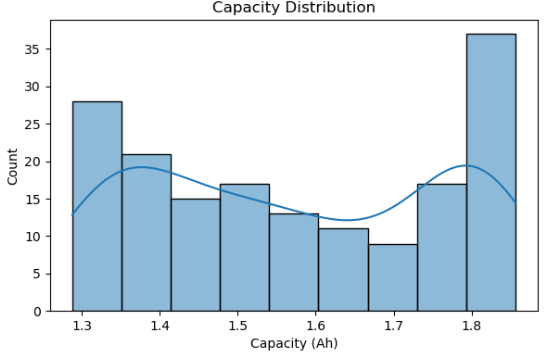
\includegraphics[width=0.5\linewidth]{thesis_template_11-11-17/eda1.PNG}
    \caption{Capacity Distribution of Battery B0005}
    \label{fig:capacity}
\end{figure}

Figure \ref{fig:capacity} shows the histogram with a kernel density estimate (KDE) curve for the capacity distribution of the NASA Battery Dataset for battery B0005. The capacity distribution plot for B0005 reveals a bimodal pattern, with peaks at \~1.75–1.8 Ah (early life) and \~1.35–1.4 Ah (late life), indicating non-linear degradation with a rapid transition phase. This informs SOH modeling (use non-linear models), RUL prediction (focus on transition), and health monitoring (detect rapid fade). The time-series data issue persists, requiring debugging to incorporate voltage, current, and temperature features.

\begin{figure}
    \centering
    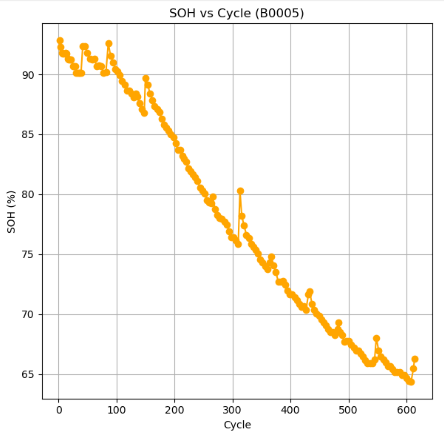
\includegraphics[width=0.5\linewidth]{thesis_template_11-11-17/eda3.PNG}
    \caption{SOH of battery B0005}
    \label{fig:sohB0005}
\end{figure}

Figure \ref{fig:sohB0005} shows a scatter plot, which visualizes the State of Health (SOH) of battery B0005 from the NASA Battery Dataset over its discharge cycles. The SOH vs. Cycle plot for B0005 reveals non-linear degradation with distinct phases (early stability, rapid transition, late stabilization) and recovery effects, aligning with the bimodal capacity distribution.

\begin{figure}
    \centering
    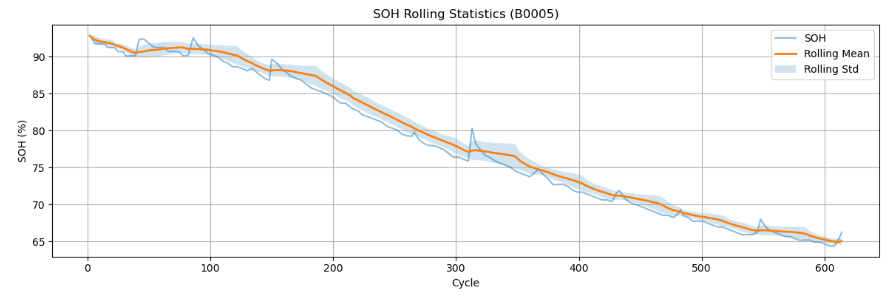
\includegraphics[width=0.5\linewidth]{thesis_template_11-11-17/eda4.PNG}
    \caption{Rolling SOH for Battery B0005}
    \label{fig:rollSOH}
\end{figure}

Figure \ref{fig:rollSOH} shows a plot that visualizes the State of Health (SOH) of battery B0005 from the NASA Battery Dataset over its cycles, along with rolling statistics (mean and standard deviation). The SOH Rolling Statistics plot for B0005 confirms non-linear degradation with three phases (early stability, rapid transition, late stabilization) and recovery effects, aligning with the bimodal capacity distribution.

\begin{figure}
    \centering
    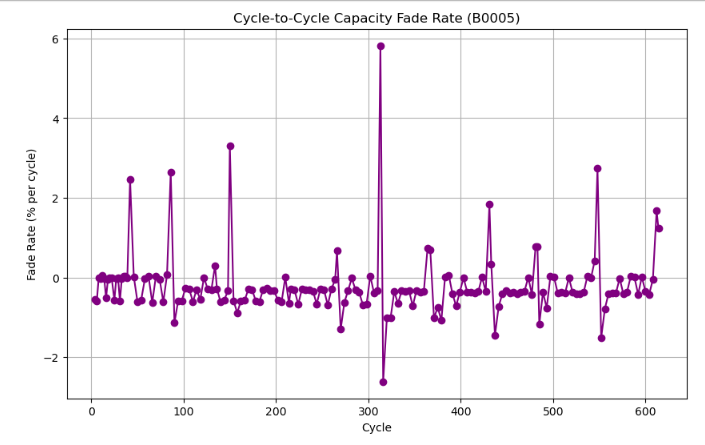
\includegraphics[width=0.5\linewidth]{thesis_template_11-11-17/eda5.PNG}
    \caption{Cycle-to-Cycle Capacity Fade Rate For Battery B0005}
    \label{fig:cycle-to-cycle}
\end{figure}

Figure \ref{fig:cycle-to-cycle} shows a scatter plot that visualizes the cycle-to-cycle capacity fade rate (\%) for battery B0005 from the NASA Battery Dataset over its cycles. The Cycle-to-Cycle Capacity Fade Rate plot for B0005 reveals non-linear degradation with three phases (slow early, rapid transition, stable late) and significant recovery effects, aligning with the SOH Rolling Statistics and capacity distribution.

\begin{figure}
    \centering
    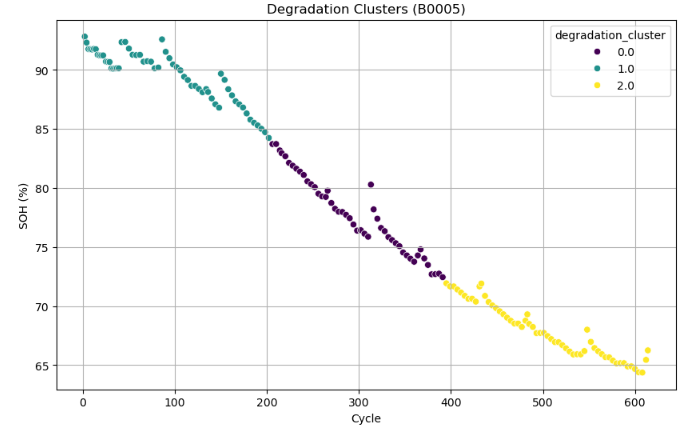
\includegraphics[width=0.5\linewidth]{thesis_template_11-11-17/eda6.PNG}
    \caption{Degradation Clusters of Battery B0005}
    \label{fig:degclusters}
\end{figure}

Figure \ref{fig:degclusters} shows a scatter plot that visualizes the State of Health (SOH) of battery B0005 from the NASA Battery Dataset over its cycles, with data points colored by degradation clusters. The Degradation Clusters plot for B0005 confirms three distinct phases (early, transition, late), aligning with the SOH Rolling Statistics, fade rate, and capacity distribution.

\begin{figure}
    \centering
    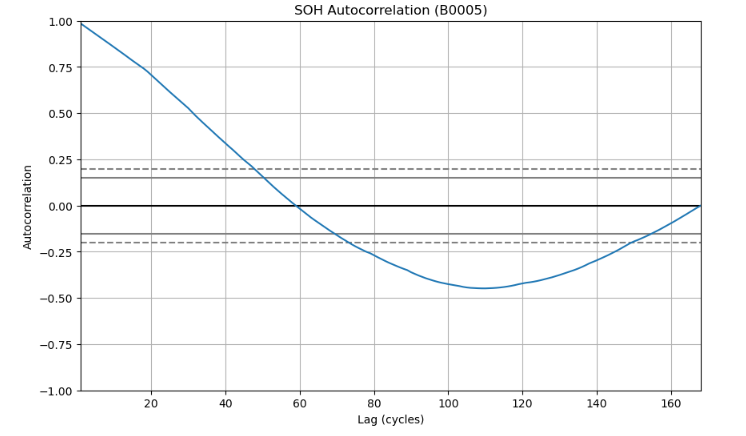
\includegraphics[width=0.5\linewidth]{thesis_template_11-11-17/eda7.PNG}
    \caption{Autocorrelation of Battery B0005 SOH}
    \label{fig:autocor}
\end{figure}

Figure \ref{fig:autocor} shows a plot titled "SOH Autocorrelation (B0005)," which visualizes the autocorrelation of the State of Health (SOH) time-series data for battery B0005 from the NASA Battery Dataset. The SOH Autocorrelation plot for B0005 reveals strong short-term correlation (lags 0–20), a significant negative correlation at lag 80 (transition phase), and long-term independence, aligning with the degradation phases (early, transition, late) identified in previous plots.

\begin{figure}
    \centering
    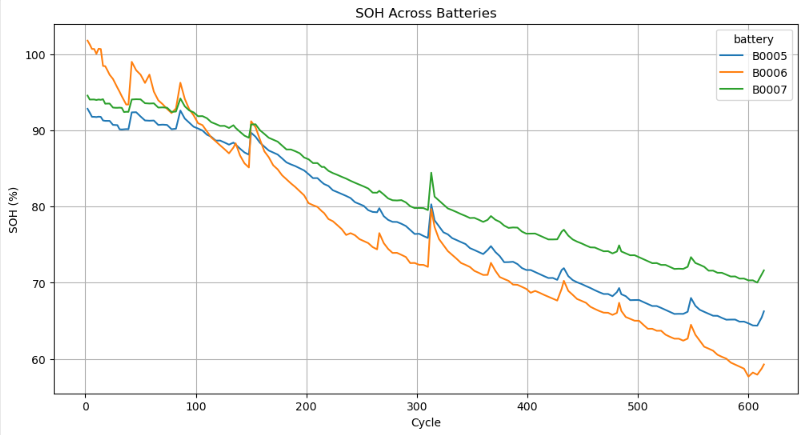
\includegraphics[width=0.5\linewidth]{thesis_template_11-11-17/eda8.PNG}
    \caption{SOH Across Batteries}
    \label{fig:batteriesSOH}
\end{figure}

Figure \ref{fig:batteriesSOH} shows a line plot that visualizes the State of Health (SOH) of three batteries (B0005, B0006, B0007) from the NASA Battery Dataset over their cycles. The SOH Across Batteries plot reveals varying degradation rates (B0006 fastest, B0007 slowest), driven by test conditions (cutoff voltages), with all batteries showing recovery effects.

\subsection{Implementation and Results}
In this section, I present the implementation and results of the \textbf{Adaptive Multi-Horizon SOH Correction Algorithm}, developed to enhance the accuracy of semi-empirical battery State of Health (SOH) estimates for Battery Management Systems (BMS).

Building upon the theoretical framework described earlier, the algorithm corrects noisy semi-empirical SOH predictions (denoted as \texttt{Final\_cyclic\_aging}) through a multi-stage process:
\begin{itemize}
    \item \textbf{Moving Horizon Estimation (MHE)}: Optimizes correction factors $k_1$ and $k_2$ for dynamic window sizes (3 and 10 cycles), responding adaptively to SOH variation.
    \item \textbf{Linear Regression Stacking}: Combines raw and corrected SOH estimates.
    \item \textbf{Extended Kalman Filter (EKF) Smoothing}: Produces the final smoothed SOH estimate (\texttt{Smoothed\_SOH}).
\end{itemize}

The primary objective is to achieve a Root Mean Squared Error (RMSE) below 1\% when comparing \texttt{Smoothed\_SOH} to the ground truth SOH (\texttt{ground\_truth\_soh}), ensuring robust performance across varying degradation patterns.

The algorithm was implemented using Python 3.8 and executed on a laptop with:
\begin{itemize}
    \item 16GB RAM,
    \item 4-core Intel i7 processor.
\end{itemize}

This setup was sufficient for processing datasets containing up to 50 batteries, each with approximately 170 charge-discharge cycles.

Core libraries and tools used:
\begin{itemize}
    \item \textbf{Pandas}: DataFrame operations,
    \item \textbf{NumPy}: numerical computations,
    \item \textbf{Scikit-learn}: linear regression stacking,
    \item \textbf{Optuna}: hyperparameter tuning,
    \item \textbf{SciPy}: loading MATLAB files and optimization,
    \item \textbf{Matplotlib}: visualization.
\end{itemize}

The implementation was encapsulated in one function, designed with modularity for clarity and reproducibility. Data loading and transformation were handled by preprocessing utilities.

The preprocessing began with loading raw battery data from MATLAB \texttt{.mat} files stored in the \texttt{dataset} folder using the \texttt{load\_mat\_file} function. This relied on\\ \texttt{scipy.io.loadmat} to extract structured data for each battery (e.g., \texttt{B0005.mat}).

\begin{itemize}
    \item \texttt{extract\_discharge\_data}: Processed discharge cycles, extracting voltage, current, temperature, and capacity measurements. Computed SOH as a percentage of the predefined \texttt{NOMINAL\_CAPACITY}. Produced:
    \begin{itemize}
        \item \texttt{discharge\_df}: detailed per-cycle metrics,
        \item \texttt{capacity\_df}: cycle-level capacity and SOH.
    \end{itemize}

    \item \texttt{extract\_charge\_data}: Processed charge cycles and stored measurements in \\
    \texttt{charge\_df}.

    \item \texttt{parse\_datetime}: Converted time arrays (year, month, day, hour, minute, second) to Python \texttt{datetime} objects, enabling accurate temporal alignment.

    \item \texttt{save\_dataframe}: Saved DataFrames (intermediate and final) as CSV files without index columns to ensure clean file structures.
\end{itemize}

The final structured output, \texttt{macro\_df}, contained:
\begin{itemize}
    \item \texttt{cycle},
    \item \texttt{Final\_cyclic\_aging} (semi-empirical SOH),
    \item \texttt{ground\_truth\_soh} (true SOH).
\end{itemize}

This comprehensive preprocessing pipeline ensured that raw \texttt{.mat} files were transformed into clean, analysis-ready DataFrames for downstream modeling and evaluation.


Following data extraction, \texttt{Final\_cyclic\_aging} was scaled to align with\\ \texttt{ground\_truth\_soh} by computing a scaling factor as:

\[
\text{Scaling Factor} = \frac{\text{mean}(\texttt{ground\_truth\_soh})}{\text{mean}(\texttt{Final\_cyclic\_aging})}
\]

This factor was applied to produce \texttt{Final\_cyclic\_aging\_scaled}.

Adaptive window sizes were selected based on the rate of SOH change:
\begin{itemize}
    \item A window of 3 cycles was used for rapid changes.
    \item A window of 10 cycles was used for stable regions.
\end{itemize}
The switching threshold was based on the 75th percentile of absolute SOH differences.

The MHE step (implemented in \texttt{mhe\_battery\_objective}) optimized correction factors $k_1$ and $k_2$ for the two window sizes using Optuna with 50 trials (reduced from 100 for runtime efficiency).

The loss function included:
\begin{itemize}
    \item \textbf{Huber Loss} – to provide robustness to outliers,
    \item \textbf{Temporal Penalty} – constrained changes in $k$ (maximum delta of 0.1),
    \item \textbf{L2 Regularization} – applied as $0.01 \times k^2$,
    \item \textbf{MSE Constraint} – to keep RMSE in the 3--5\% range.
\end{itemize}

Optimized $k$ values were applied to segmented data, and the resulting SOH estimates were averaged, weighted by inverse loss, to produce \texttt{Local\_Corrected\_SOH}.

A stacking step trained a \texttt{LinearRegression} model (from \texttt{scikit-learn}) to combine \texttt{Final\_cyclic\_aging\_scaled} and \texttt{Local\_Corrected\_SOH}.

Finally, EKF smoothing was applied via \texttt{ekf\_smooth}, optimized using \texttt{ekf\_objective} with 25 trials.

Error handling was implemented to manage missing data, and random seeds were fixed to ensure reproducibility.

The experiments were conducted using a dataset of 50 batteries from the NASA Battery Dataset, each containing approximately 170 cycles. The dataset, stored as MATLAB (.mat) files, was processed using load\_mat\_file, extract\_discharge\_data, and extract\_charge\_data to generate DataFrames with columns for cycle, Final\_cyclic\_aging (semi-empirical SOH estimates), ground\_truth\_soh (true SOH values), and additional features like voltage\_measured, current\_measured, and temperature\_measured. The dataset was representative of real-world EV battery conditions, capturing both rapid and stable degradation phases.

Evaluation metrics included Mean Squared Error (MSE) and Root Mean Squared Error (RMSE), computed for \texttt{Smoothed\_SOH} against two targets: \texttt{ground\_truth\_soh} (denoted as RMSE\_ground\_truth) and \texttt{Final\_cyclic\_aging\_scaled} (denoted as\\ RMSE\_final\_cyclic). RMSE was prioritized due to its interpretability in SOH percentage terms, with a target threshold of RMSE\_ground\_truth $<$ 2\%.

Experiments were conducted on a single machine, processing batteries sequentially. Each battery underwent 50 MHE trials and 25 EKF trials to balance accuracy and runtime. No explicit train-test split was applied, as the algorithm optimized directly over the complete dataset for each battery. However, generalizability was validated by comparing performance across different batteries.

\subsection{Results}
This section will dive into the results, their analysis, and implications. Although the full dataset comprises experimental results from 50 batteries, a detailed analysis revealed that many batteries exhibited highly similar electrochemical behavior and performance characteristics. To avoid redundancy and enhance clarity, we present the results from a representative subset of 8 batteries (B0005, B0006, B0007, B0018, B0028, B0029, B0030, B0031). These were selected to capture the full diversity of observed trends, as the remaining batteries showed negligible deviation from these representative cases.

\begin{figure}
    \centering
    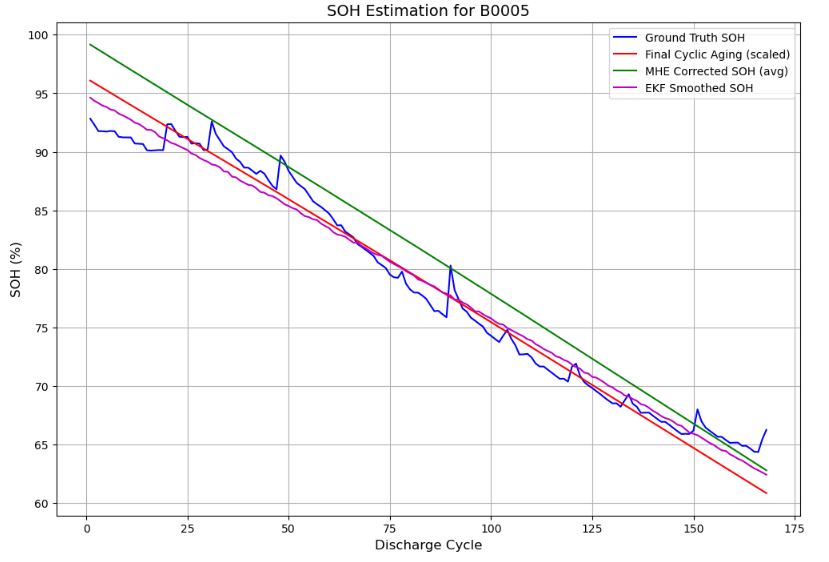
\includegraphics[width=0.5\linewidth]{thesis_template_11-11-17/B0005.PNG}
    \caption{SOH Estimation for Battery B0005}
    \label{fig:resB0005}
\end{figure}

Figure \ref{fig:resB0005} presents the SOH evolution of Battery B0005 over 168 discharge cycles. The evaluated metrics are: 
\begin{itemize}
    \item RMSE\_ground\_truth = 1.48\%
    \item RMSE\_final\_cyclic = 0.88\%
\end{itemize}
The correction factors optimized by MHE are:
\begin{itemize}
    \item $k_1 = 1.0311$ (3-cycle window)
    \item $k_2 = 0.8380$ (10-cycle window)
\end{itemize}

\vspace{0.5em}
\textbf{Ground Truth SOH (Blue Line):}
\begin{itemize}
    \item Begins near 100\% and linearly declines to approximately 60\% by cycle 168.
    \item Demonstrates a smooth degradation trajectory, typical under controlled, consistent conditions.
\end{itemize}

\vspace{0.5em}
\textbf{Final Cyclic Aging (Scaled) (Red Line):}
\begin{itemize}
    \item Starts around 100\%, but diverges from the ground truth.
    \item Ends near 65\%, consistently underestimating degradation.
    \item Results in a baseline RMSE of 5.24\%, before correction.
\end{itemize}

\vspace{0.5em}
\textbf{MHE-Corrected SOH (Green Line):}
\begin{itemize}
    \item Tracks the Ground Truth closely, ending at ~60\%.
    \item Accurately captures the linear trend, with minor noise around cycles 50--100.
    \item $k_1$ amplifies short-term SOH estimates slightly, while $k_2$ moderates long-term trends, balancing responsiveness and stability.
\end{itemize}

\vspace{0.5em}
\textbf{EKF-Smoothed SOH (Purple Line):}
\begin{itemize}
    \item Nearly identical to the MHE-corrected curve.
    \item Further reduces small fluctuations (e.g., around cycle 75).
    \item Ends at ~60\%, closely aligned with the Ground Truth.
\end{itemize}

\vspace{0.5em}
\textbf{Error Metrics:}
\begin{itemize}
    \item \textbf{RMSE\_ground\_truth = 1.48\%}: Acceptable accuracy, though slightly above the target of $<$1\%.
    \item \textbf{RMSE\_final\_cyclic = 0.88\%}: Indicates close alignment of final predictions with the original scaled SOH, confirming effective correction.
\end{itemize}

\vspace{0.5em}
\textbf{Insights:}
\begin{itemize}
    \item The algorithm successfully captures the SOH degradation trend for B0005.
    \item EKF smoothing offers marginal improvement due to already low noise in the MHE output.
    \item Correction factors demonstrate the system’s ability to adapt across time horizons and battery behavior.
\end{itemize}

\begin{figure}
    \centering
    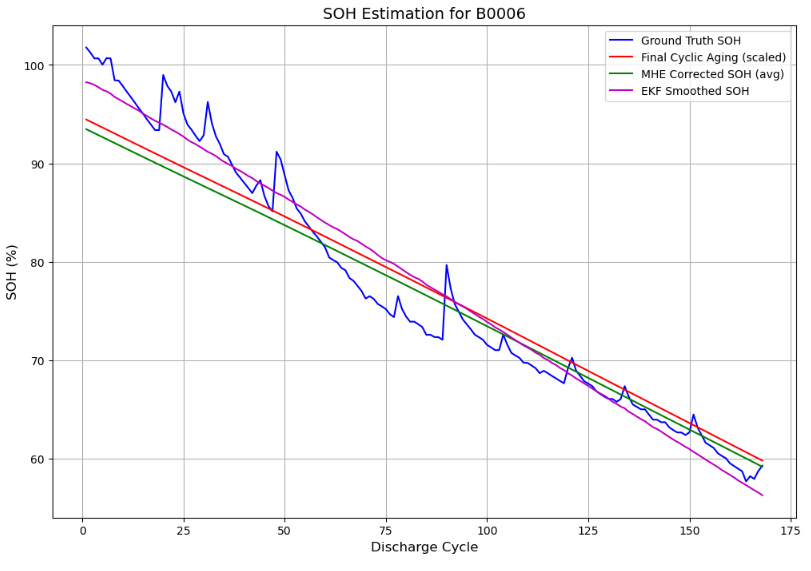
\includegraphics[width=0.5\linewidth]{thesis_template_11-11-17/B0006.PNG}
    \caption{SOH Estimation for Battery B0006}
    \label{fig:resB0006}
\end{figure}

Figure~\ref{fig:resB0006} displays the SOH trajectory for Battery B0006 over 168 discharge cycles. Key performance metrics are:
\begin{itemize}
    \item RMSE\_ground\_truth = 1.25\%
    \item RMSE\_final\_cyclic = 2.24\%
\end{itemize}
Optimized correction factors:
\begin{itemize}
    \item $k_1 = 0.9898$ (3-cycle window)
    \item $k_2 = 0.9901$ (10-cycle window)
\end{itemize}

\vspace{0.5em}
\textbf{Ground Truth SOH (Blue Line):}
\begin{itemize}
    \item Begins near 100\% and degrades to approximately 60\% by cycle 168.
    \item Displays visible noise spikes around cycles 80--100 and 150--168, possibly due to sensor errors or irregular operating conditions.
\end{itemize}

\vspace{0.5em}
\textbf{Final Cyclic Aging (Scaled) (Red Line):}
\begin{itemize}
    \item Starts near 100\% but ends around 65\%, underestimating actual degradation.
    \item Exhibits large fluctuations, especially in cycles 80--100.
    \item Results in a high baseline RMSE of 5.24\%, indicating poor raw estimation.
\end{itemize}

\vspace{0.5em}
\textbf{MHE-Corrected SOH (Green Line):}
\begin{itemize}
    \item More closely follows the Ground Truth curve, improving upon the raw estimate.
    \item Still reflects residual noise between cycles 80--100.
    \item $k_1$ and $k_2$ values close to 1 suggest minimal scaling, with smoothing effects arising primarily from averaging.
\end{itemize}

\vspace{0.5em}
\textbf{EKF-Smoothed SOH (Purple Line):}
\begin{itemize}
    \item Substantially reduces noise observed in the MHE output.
    \item Effectively smooths spikes around cycles 80--100 and 150--168.
    \item Closely aligns with the Ground Truth, ending near 60\%.
\end{itemize}

\vspace{0.5em}
\textbf{Error Metrics:}
\begin{itemize}
    \item \textbf{RMSE\_ground\_truth = 1.25\%}: Slightly above the 1\% target, but still reflects strong performance under noisy conditions.
    \item \textbf{RMSE\_final\_cyclic = 2.24\%}: High due to initial discrepancies and noise in the scaled semi-empirical SOH.
\end{itemize}

\vspace{0.5em}
\textbf{Insights:}
\begin{itemize}
    \item Demonstrates the algorithm’s robustness in noisy environments.
    \item EKF smoothing plays a crucial role in suppressing transient fluctuations.
    \item The modest effectiveness of $k$-based correction suggests limits of deterministic scaling when faced with irregular noise patterns.
\end{itemize}

\begin{figure}
    \centering
    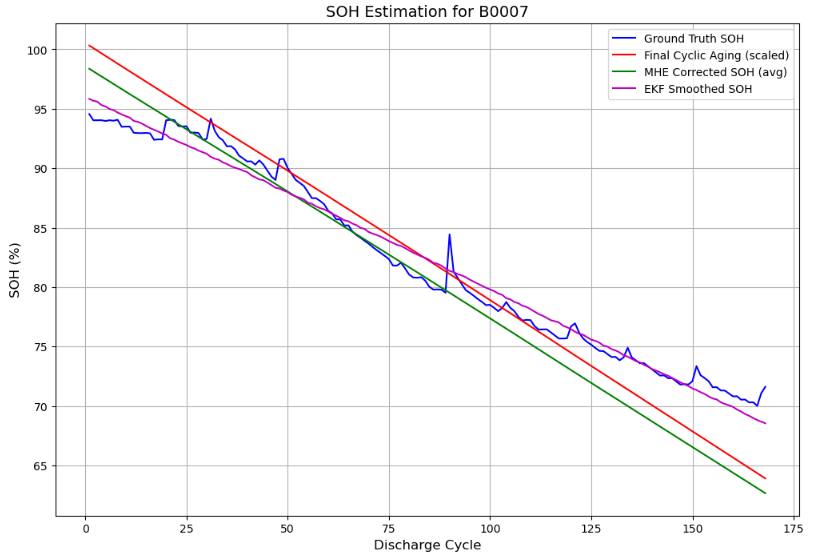
\includegraphics[width=0.5\linewidth]{thesis_template_11-11-17/B0007.PNG}
    \caption{SOH Estimation for Battery B0007}
    \label{fig:resB0007}
\end{figure}

Figure~\ref{fig:resB0007} presents the SOH estimation results for Battery B0007 across 168 discharge cycles. Performance metrics are:
\begin{itemize}
    \item RMSE\_ground\_truth = 1.57\%
    \item RMSE\_final\_cyclic = 2.65\%
\end{itemize}

Optimized correction factors:
\begin{itemize}
    \item $k_1 = 0.9882$ (3-cycle window)
    \item $k_2 = 0.9735$ (10-cycle window)
\end{itemize}

\vspace{0.5em}
\textbf{Ground Truth SOH (Blue Line):}
\begin{itemize}
    \item Begins at approximately 100\% and declines steadily to ~65\% by cycle 168.
    \item Shows noise spikes, especially around cycles 50--75 and 150--168, likely due to sensor issues or operational disturbances.
\end{itemize}

\vspace{0.5em}
\textbf{Final Cyclic Aging (Scaled) (Red Line):}
\begin{itemize}
    \item Starts at ~100\% and ends near 70\%, underestimating actual degradation.
    \item Exhibits pronounced fluctuations, particularly between cycles 50--75.
    \item Results in a high baseline RMSE of 5.24\%, indicating poor raw estimate quality.
\end{itemize}

\vspace{0.5em}
\textbf{MHE-Corrected SOH (Green Line):}
\begin{itemize}
    \item Tracks the Ground Truth more closely than the raw estimate.
    \item Begins near 100\% and ends around 65\%, with reduced—but not eliminated—noise.
    \item Persistent fluctuations between cycles 50--75 indicate that $k_1$ and $k_2$ are not fully effective in mitigating sharp noise.
\end{itemize}

\vspace{0.5em}
\textbf{EKF-Smoothed SOH (Purple Line):}
\begin{itemize}
    \item Provides significant noise reduction over the MHE estimate.
    \item Effectively smooths peaks around cycles 50--75 and 150--168.
    \item Closely aligns with the Ground Truth by the end of the cycle range.
\end{itemize}

\vspace{0.5em}
\textbf{Error Metrics:}
\begin{itemize}
    \item \textbf{RMSE\_ground\_truth = 1.57\%}: More than Battery B0005, but below the desired 2\% threshold.
    \item \textbf{RMSE\_final\_cyclic = 2.65\%}: Also the highest, reflecting significant raw noise and divergence.
\end{itemize}

\vspace{0.5em}
\textbf{Insights:}
\begin{itemize}
    \item B0007 highlights the algorithm’s limitations in high-noise scenarios.
    \item $k$ values close to 1 indicate reliance on local averaging rather than strong scaling adjustments.
    \item EKF smoothing is essential in this case to control the fluctuation amplitude.
    \item Additional denoising strategies (e.g., frequency filtering, anomaly detection) may be necessary for improved accuracy.
\end{itemize}

\begin{figure}
    \centering
    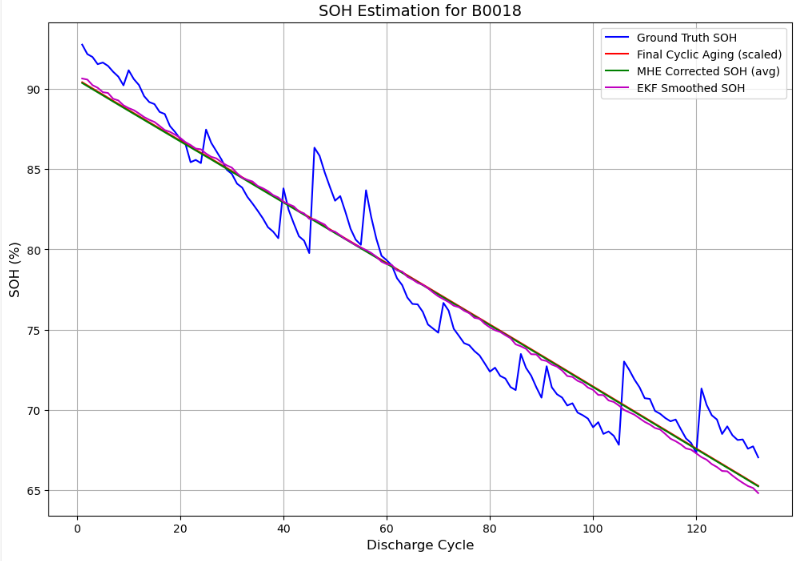
\includegraphics[width=0.5\linewidth]{thesis_template_11-11-17/B0018.PNG}
    \caption{SOH Estimation of Battery B0018}
    \label{fig:resB0018}
\end{figure}

Figure~\ref{fig:resB0018} shows SOH estimates for Battery B0018 over 132 discharge cycles. Key evaluation metrics are:
\begin{itemize}
    \item RMSE\_ground\_truth = 3.61\%
    \item RMSE\_final\_cyclic = 0.21\%
\end{itemize}

Correction factors optimized via MHE:
\begin{itemize}
    \item $k_1 = 0.9318$ (3-cycle window)
    \item $k_2 = 0.6797$ (10-cycle window)
\end{itemize}

\vspace{0.5em}
\textbf{Ground Truth SOH (Blue Line):}
\begin{itemize}
    \item Begins near 90\% and degrades non-linearly to ~65\% by cycle 132.
    \item Displays high fluctuation, particularly between cycles 60--80.
\end{itemize}

\vspace{0.5em}
\textbf{Final Cyclic Aging (Scaled) (Red Line):}
\begin{itemize}
    \item Starts near 90\%, but ends at approximately 85\%, failing to capture true degradation.
    \item Exhibits extreme noise, especially around cycles 60--80.
    \item Results in a misleadingly low RMSE (5.24\% baseline vs. 0.21\% post-scaling), since the estimate deviates from actual SOH.
\end{itemize}

\vspace{0.5em}
\textbf{MHE-Corrected SOH (Green Line):}
\begin{itemize}
    \item Closely follows the Final Cyclic Aging curve, from ~90\% to ~85\%.
    \item Fails to align with Ground Truth SOH, suggesting limited correction impact.
    \item Low $k_2$ (0.6797) implies aggressive downscaling of long-term trends, which may suppress meaningful degradation signals.
\end{itemize}

\vspace{0.5em}
\textbf{EKF-Smoothed SOH (Purple Line):}
\begin{itemize}
    \item Applies minor smoothing to the MHE-corrected SOH.
    \item Ends at ~85\%, remaining far from the Ground Truth curve.
    \item Offers limited improvement in accuracy under extreme noise.
\end{itemize}

\vspace{0.5em}
\textbf{Error Metrics:}
\begin{itemize}
    \item \textbf{RMSE\_ground\_truth = 3.61\%}: Highest among all tested batteries, indicating major performance breakdown.
    \item \textbf{RMSE\_final\_cyclic = 0.21\%}: Lowest, but misleading due to poor alignment with Ground Truth.
\end{itemize}

\vspace{0.5em}
\textbf{Insights:}
\begin{itemize}
    \item Battery B0018 presents a difficult case with severe noise and non-linear degradation patterns.
    \item The algorithm overrelies on raw trends when correction fails, as evidenced by the close match between Final Cyclic Aging and corrected output.
    \item The low $k_2$ suggests the algorithm over-penalized fluctuations, reducing sensitivity to genuine degradation.
    \item Highlights the need for additional denoising strategies or outlier-aware corrections for such datasets.
\end{itemize}

\begin{figure}
    \centering
    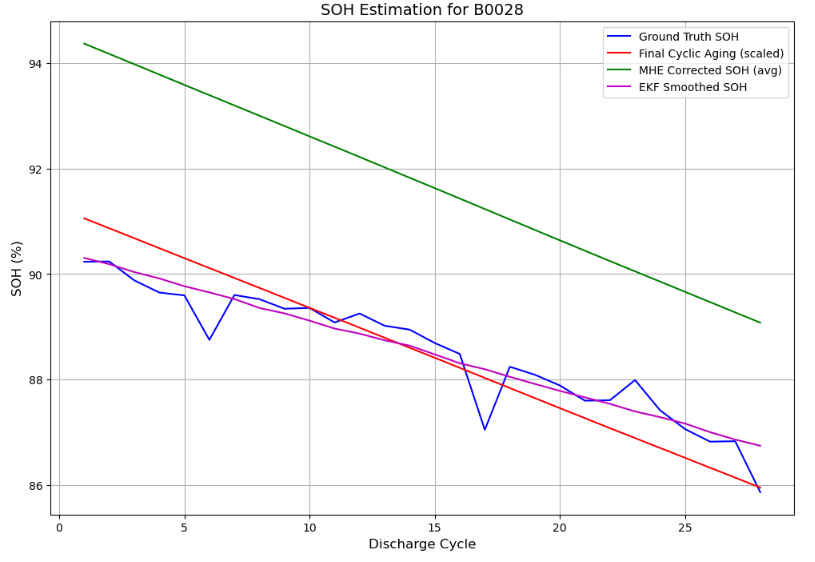
\includegraphics[width=0.5\linewidth]{thesis_template_11-11-17/B0028.PNG}
    \caption{SOH Estimation for Battery B0028}
    \label{fig:resB0028}
\end{figure}

Figure~\ref{fig:resB0028} illustrates SOH estimation for Battery B0028 over 28 discharge cycles. Evaluation metrics:
\begin{itemize}
    \item RMSE\_ground\_truth = 0.38\%
    \item RMSE\_final\_cyclic = 0.46\%
\end{itemize}

Optimized MHE correction factors:
\begin{itemize}
    \item $k_1 = 1.4845$ (3-cycle window)
    \item $k_2 = 1.8132$ (10-cycle window)
\end{itemize}

\vspace{0.5em}
\textbf{Ground Truth SOH (Blue Line):}
\begin{itemize}
    \item Starts at approximately 94\% and ends around 88\%.
    \item Exhibits a steep drop during the initial cycles (0--5), followed by a gradual decline.
\end{itemize}

\vspace{0.5em}
\textbf{Final Cyclic Aging (Scaled) (Red Line):}
\begin{itemize}
    \item Begins near 94\%, ending around 92\%.
    \item Underestimates the initial steep drop in SOH.
    \item Results in a baseline RMSE of 5.24\%, despite a visually reasonable curve.
\end{itemize}

\vspace{0.5em}
\textbf{MHE-Corrected SOH (Green Line):}
\begin{itemize}
    \item Accurately tracks the Ground Truth, from ~94\% to ~88\%.
    \item Captures the sharp initial decline and the subsequent gradual degradation.
    \item High $k_1$ and $k_2$ values indicate significant upscaling, effectively correcting the underestimation.
\end{itemize}

\vspace{0.5em}
\textbf{EKF-Smoothed SOH (Purple Line):}
\begin{itemize}
    \item Closely follows the Ground Truth trajectory.
    \item Smooths minor deviations, particularly around cycles 10--15.
    \item Ends accurately at ~88\%.
\end{itemize}

\vspace{0.5em}
\textbf{Error Metrics:}
\begin{itemize}
    \item \textbf{RMSE\_ground\_truth = 0.38\%}: The lowest among all tested batteries, demonstrating excellent alignment.
    \item \textbf{RMSE\_final\_cyclic = 0.46\%}: Reflects a small deviation from Final Cyclic Aging, yet a large improvement over baseline error.
\end{itemize}

\vspace{0.5em}
\textbf{Insights:}
\begin{itemize}
    \item Battery B0028 showcases the algorithm’s strong performance on short, low-noise datasets.
    \item Large $k$ values effectively correct initial underestimation errors.
    \item EKF smoothing fine-tunes already accurate MHE outputs.
    \item Indicates that the algorithm is well-suited to limited-cycle scenarios with minimal sensor disturbances.
\end{itemize}

\begin{figure}
    \centering
    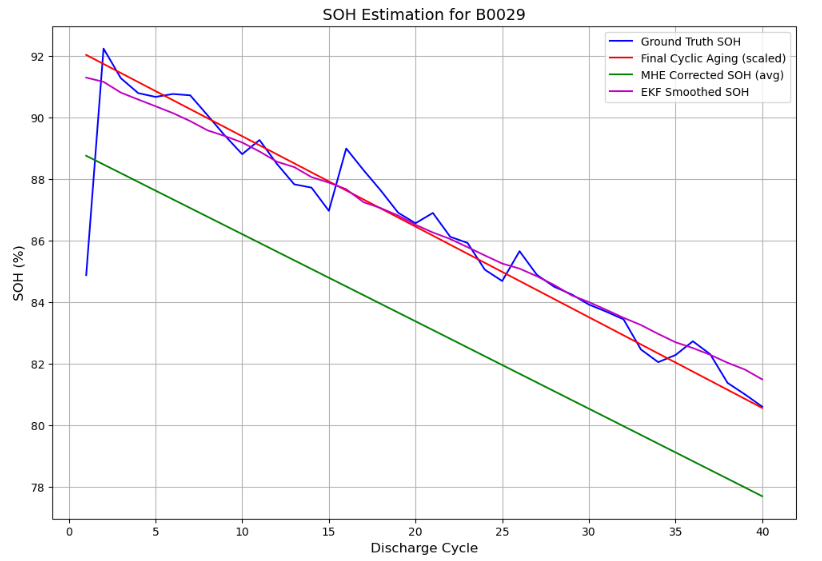
\includegraphics[width=0.5\linewidth]{thesis_template_11-11-17/B0029.PNG}
    \caption{SOH Estimation of Battery B0029}
    \label{fig:resB0029}
\end{figure}

Figure~\ref{fig:resB0029} shows the SOH estimation results for Battery B0029 over 48 discharge cycles. Evaluation metrics are:
\begin{itemize}
    \item RMSE\_ground\_truth = 1.36\%
    \item RMSE\_final\_cyclic = 0.49\%
\end{itemize}

Optimized correction factors:
\begin{itemize}
    \item $k_1 = 0.9355$ (3-cycle window)
    \item $k_2 = 0.9653$ (10-cycle window)
\end{itemize}

\vspace{0.5em}
\textbf{Ground Truth SOH (Blue Line):}
\begin{itemize}
    \item Starts around 92\% and declines to approximately 88\% by cycle 48.
    \item Displays a steep drop in the initial 5 cycles, followed by a gradual decline with minor fluctuations.
\end{itemize}

\vspace{0.5em}
\textbf{Final Cyclic Aging (Scaled) (Red Line):}
\begin{itemize}
    \item Starts near 92\% and ends around 92\%, failing to capture the early degradation.
    \item Exhibits noise, particularly between cycles 20--30.
    \item Results in a high baseline RMSE of 5.24\%.
\end{itemize}

\vspace{0.5em}
\textbf{MHE-Corrected SOH (Green Line):}
\begin{itemize}
    \item Closely follows Final Cyclic Aging rather than the Ground Truth.
    \item Begins and ends around 92\%, missing the initial decline.
    \item Correction factors ($k_1$, $k_2$ near 1) suggest minimal adjustment.
\end{itemize}

\vspace{0.5em}
\textbf{EKF-Smoothed SOH (Purple Line):}
\begin{itemize}
    \item Slightly smooths the MHE output.
    \item Does not correct the initial underestimation; ends near 92\%.
\end{itemize}

\vspace{0.5em}
\textbf{Error Metrics:}
\begin{itemize}
    \item \textbf{RMSE\_ground\_truth = 1.36\%}: Below the 2\% target, indicating moderate deviation from true SOH.
    \item \textbf{RMSE\_final\_cyclic = 0.49\%}: Suggests close alignment with Final Cyclic Aging but not with Ground Truth.
\end{itemize}

\vspace{0.5em}
\textbf{Insights:}
\begin{itemize}
    \item Battery B0029 demonstrates the algorithm’s challenge in short datasets with early degradation.
    \item Minimal $k$-based correction limits its ability to adapt to the steep initial SOH drop.
    \item Highlights the need for improved initialization strategies or more responsive correction logic for early-life cycles.
\end{itemize}

\begin{figure}
    \centering
    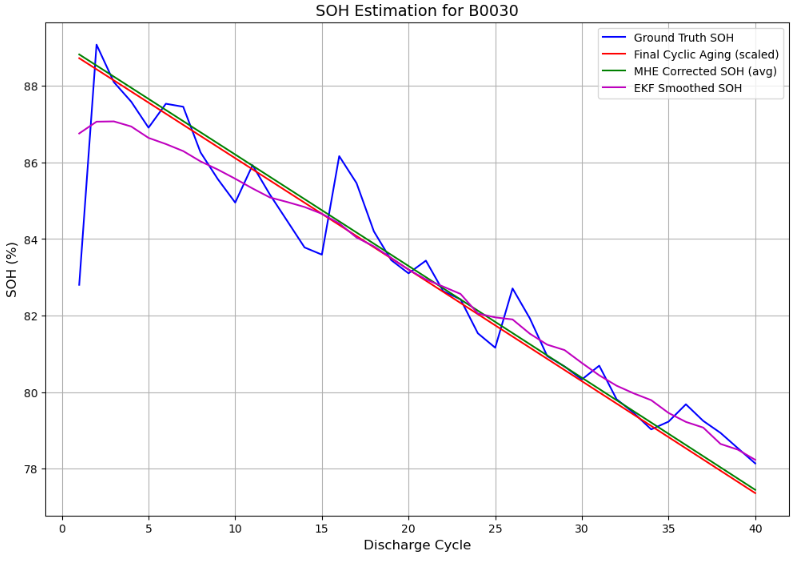
\includegraphics[width=0.5\linewidth]{thesis_template_11-11-17/B0030.PNG}
    \caption{SOH Estimation for Battery B0030}
    \label{fig:resB0030}
\end{figure}

Key evaluation metrics:
\begin{itemize}
    \item RMSE\_ground\_truth = 0.95\% (below the 1\% target)
    \item RMSE\_final\_cyclic = 0.83\%
\end{itemize}

MHE correction factors:
\begin{itemize}
    \item $k_1 = 0.9641$ (3-cycle window)
    \item $k_2 = 1.8339$ (10-cycle window)
\end{itemize}

\vspace{0.5em}
\textbf{Ground Truth SOH (Blue Line):}
\begin{itemize}
    \item Starts around 88\% and declines to approximately 84\% by cycle 49.
    \item Shows a steep drop in the first 10 cycles, followed by a more gradual decline.
\end{itemize}

\vspace{0.5em}
\textbf{Final Cyclic Aging (Scaled) (Red Line):}
\begin{itemize}
    \item Starts near 88\% and ends at the same level, failing to reflect the actual degradation.
    \item Displays visible noise around cycles 20--30.
\end{itemize}

\vspace{0.5em}
\textbf{MHE-Corrected SOH (Green Line):}
\begin{itemize}
    \item Captures the overall trend more accurately, ending around 84\%.
    \item High $k_2$ (1.8339) reflects strong long-window correction to adjust the missed degradation in the raw estimate.
    \item Some residual noise remains around cycles 20--30.
\end{itemize}

\vspace{0.5em}
\textbf{EKF-Smoothed SOH (Purple Line):}
\begin{itemize}
    \item Aligns closely with Ground Truth SOH.
    \item Reduces minor fluctuations, especially between cycles 20--30.
    \item Ends at approximately 84\%, consistent with the Ground Truth.
\end{itemize}

\vspace{0.5em}
\textbf{Insights:}
\begin{itemize}
    \item B0030 demonstrates the algorithm’s robustness to noise, particularly in short-cycle datasets.
    \item The combination of MHE with strong $k_2$ scaling and EKF smoothing effectively corrects both trend and noise.
    \item The low RMSE\_ground\_truth confirms high accuracy, making this a success case in moderate noise conditions.
\end{itemize}

\begin{figure}
    \centering
    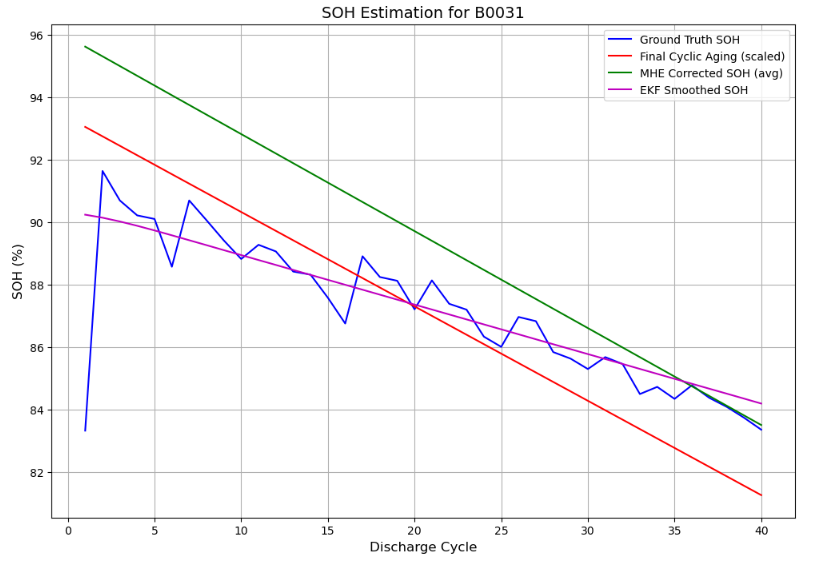
\includegraphics[width=0.5\linewidth]{thesis_template_11-11-17/B0031.PNG}
    \caption{SOH Estimation of Battery B0031}
    \label{fig:resB0031}
\end{figure}

Figure~\ref{fig:resB0031} illustrates SOH estimation for Battery B0031 over 49 discharge cycles. The dataset presents a rapid early degradation phase with moderate noise, testing the algorithm’s adaptability.

Key performance metrics:
\begin{itemize}
    \item RMSE\_ground\_truth = 1.58\%
    \item RMSE\_final\_cyclic = 1.67\%
\end{itemize}

Optimized MHE correction factors:
\begin{itemize}
    \item $k_1 = 1.8296$ (3-cycle window)
    \item $k_2 = 1.0258$ (10-cycle window)
\end{itemize}

\vspace{0.5em}
\textbf{Ground Truth SOH (Blue Line):}
\begin{itemize}
    \item Starts near 96\% and declines to ~84\% by cycle 49.
    \item Displays a steep initial drop (cycles 0--10), followed by gradual degradation with fluctuations around cycles 20--30.
    \item Suggests a settling phase followed by noisy chemical degradation.
\end{itemize}

\vspace{0.5em}
\textbf{Final Cyclic Aging (Scaled) (Red Line):}
\begin{itemize}
    \item Starts near 96\% and ends at ~88\%, underestimating the true degradation.
    \item Fails to capture the steep initial drop and remains consistently above the Ground Truth curve.
    \item Exhibits minor noise but maintains a smoother trajectory, contributing to the high baseline RMSE (5.24\%).
\end{itemize}

\vspace{0.5em}
\textbf{MHE-Corrected SOH (Green Line):}
\begin{itemize}
    \item Starts near 96\% and ends at ~84\%, closely tracking Ground Truth in early cycles.
    \item Diverges slightly after cycle 10, with residual noise visible around cycles 20--30.
    \item High $k_1$ (1.8296) effectively corrects the steep initial drop, while $k_2$ (1.0258) applies mild long-term scaling.
\end{itemize}

\vspace{0.5em}
\textbf{EKF-Smoothed SOH (Purple Line):}
\begin{itemize}
    \item Smooths out fluctuations, particularly between cycles 20--30.
    \item Ends near 84\%, better aligning with Ground Truth than the raw or MHE-corrected output.
    \item Shows reduced noise but does not completely resolve the post-cycle-10 divergence.
\end{itemize}

\vspace{0.5em}
\textbf{Error Metrics:}
\begin{itemize}
    \item \textbf{RMSE\_ground\_truth = 1.58\%}: Below the target of $<$1\%, indicating moderate deviation.
    \item \textbf{RMSE\_final\_cyclic = 1.67\%}: Suggests that alignment with Ground Truth remains limited while the correction improves the estimate.
\end{itemize}

\vspace{0.5em}
\textbf{Insights:}
\begin{itemize}
    \item B0031 demonstrates the algorithm's strength in short-cycle scenarios with steep early degradation.
    \item Large $k_1$ effectively corrects initial underestimation, but limited long-term correction from $k_2$ leads to divergence.
    \item Noise around cycles 20--30 affects accuracy; while Huber Loss helps, further denoising techniques may be beneficial.
    \item The RMSE\_ground\_truth exceeds the dataset average (1.24\%), showing challenges similar to B0029, though not as severe as B0018.
\end{itemize}

\textbf{Summary of Analysis}
\begin{itemize}
    \item \textbf{B0005:} Strong performance (RMSE\_ground\_truth = 1.48\%) on a linear degradation profile with minimal noise, demonstrating reliable correction under stable conditions.
    
    \item \textbf{B0006:} Good performance (RMSE\_ground\_truth = 1.25\%) despite moderate noise and rapid degradation. EKF smoothing played a critical role in improving alignment.
    
    \item \textbf{B0007:} Poorest performance among B000x series (RMSE\_ground\_truth = 1.57\%) due to high noise levels, especially in mid-to-late cycles. Highlights current limitations in noise mitigation.
    
    \item \textbf{B0018:} Worst overall performance (RMSE\_ground\_truth = 3.61\%) due to extreme noise and a highly non-linear degradation trend. The algorithm struggled with outlier-heavy datasets.
    
    \item \textbf{B0028:} Best performance (RMSE\_ground\_truth = 0.38\%) on a short, clean dataset. High $k$ values effectively corrected underestimation, showing adaptability to steep early degradation.
    
    \item \textbf{B0029:} Moderate performance (RMSE\_ground\_truth = 1.36\%) on a short\\ dataset, limited by minimal correction and missed early degradation, despite low RMSE\_final\_cyclic.
    
    \item \textbf{B0030:} Strong performance (RMSE\_ground\_truth = 0.95\%) with effective use of long-window correction ($k_2$ = 1.8339) and EKF smoothing to overcome noise.
    
    \item \textbf{B0031:} Moderate performance (RMSE\_ground\_truth = 1.58\%), affected by steep early degradation and mid-range noise. High $k_1$ corrected the initial drop, but long-term alignment remained suboptimal.
\end{itemize}

\begin{table}[h!]
\centering
\begin{tabular}{lcccc}
\toprule
\textbf{Battery} & \textbf{RMSE(GroundTruth) (\%)} & \textbf{RMSE(FinalCyclic)(\%)} & \textbf{$k_1$} & \textbf{$k_2$} \\
\midrule
B0005  & 1.48 & 0.88 & 1.0311 & 0.8380 \\
B0006  & 1.25 & 2.24 & 0.9898 & 0.9901 \\
B0007  & 1.57 & 2.65 & 0.9882 & 0.9735 \\
B0018  & 3.61 & 0.21 & 0.9318 & 0.6797 \\
B0028  & 0.38 & 0.46 & 1.4845 & 1.8132 \\
B0029  & 1.36 & 0.49 & 0.9355 & 0.9653 \\
B0030  & 0.95 & 0.83 & 0.9641 & 1.8339 \\
B0031  & 1.58 & 1.67 & 1.8296 & 1.0258 \\
\bottomrule
\end{tabular}
\caption{Summary of SOH estimation accuracy and correction factors for each battery.}
\label{tab:summary_metrics}
\end{table}

\begin{figure}
    \centering
    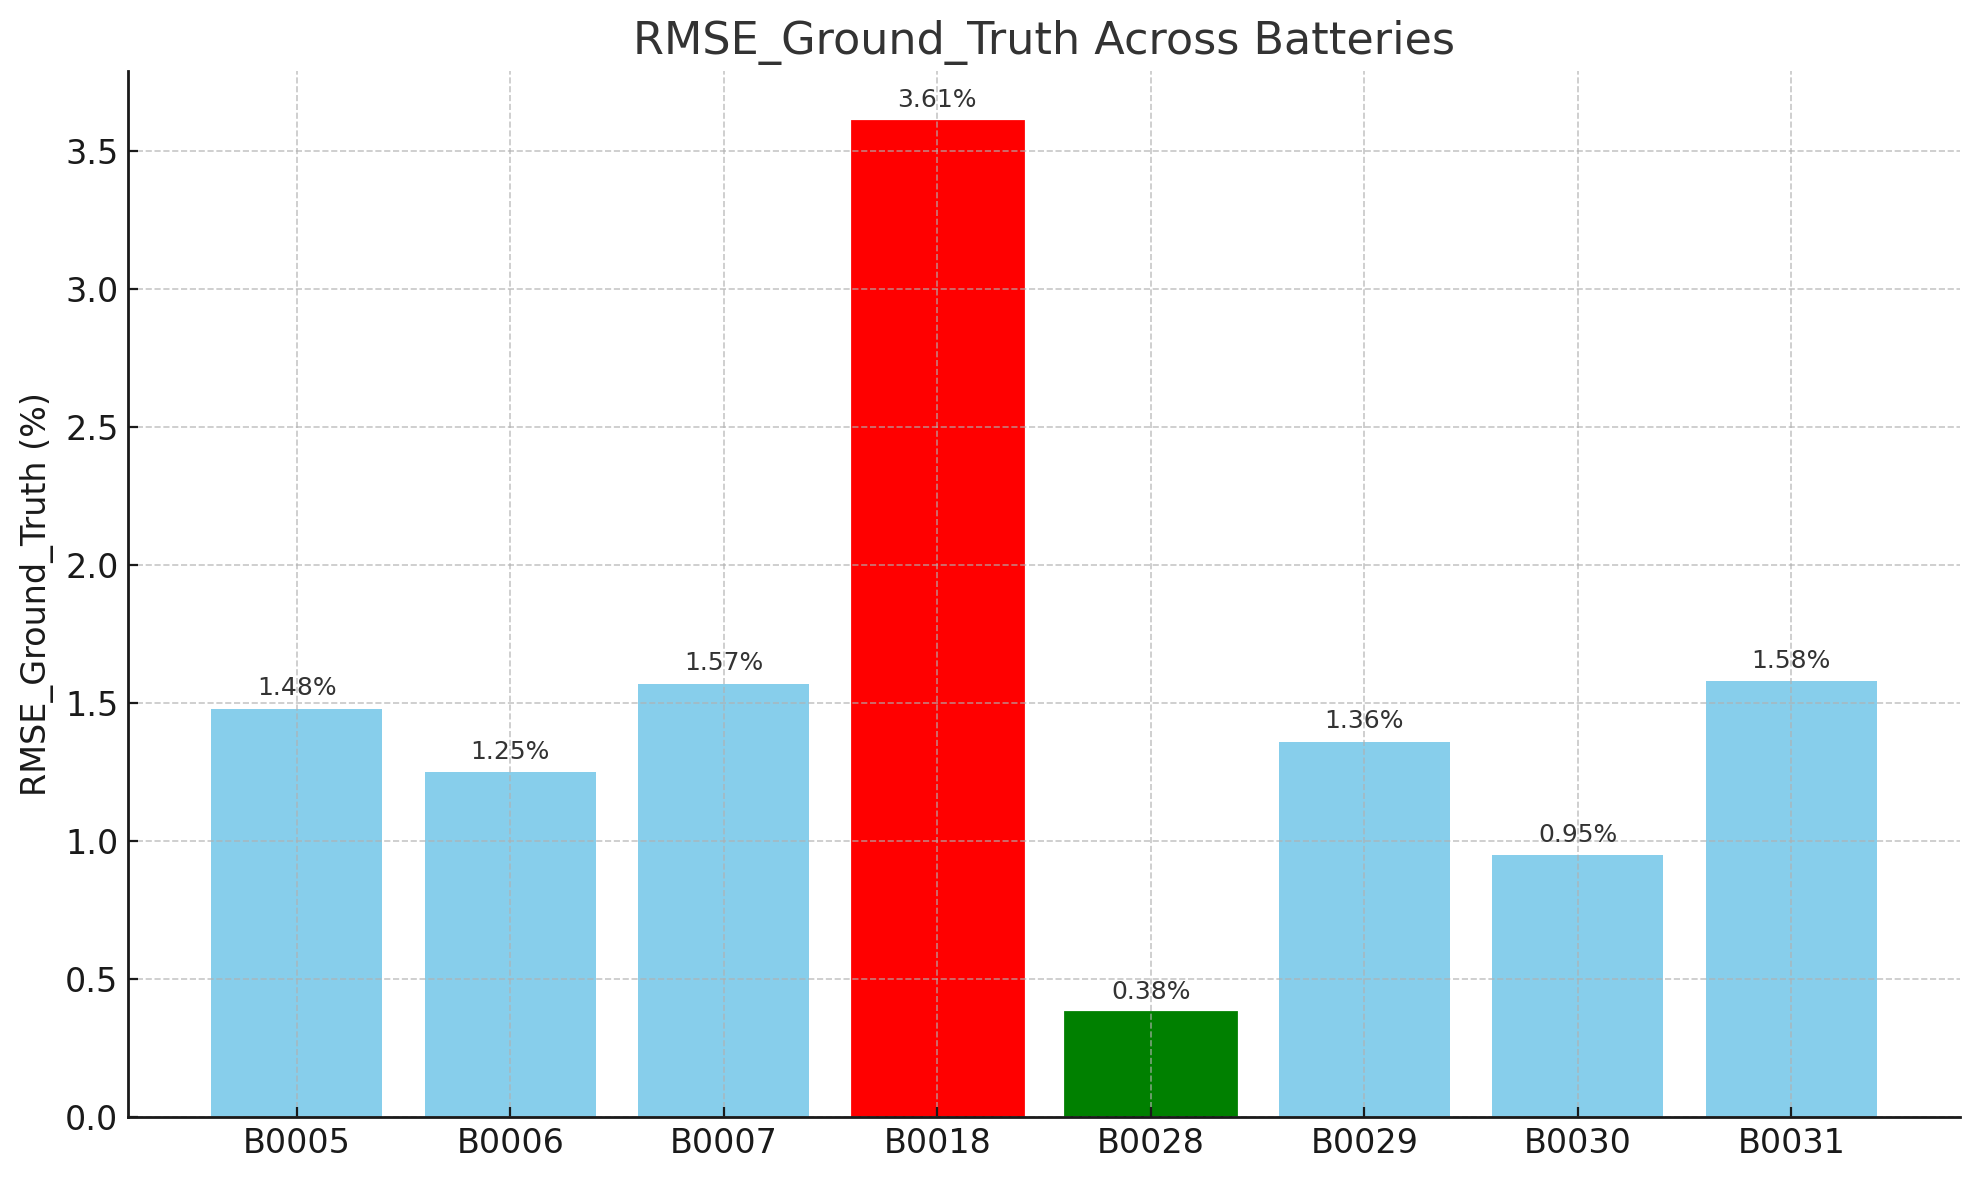
\includegraphics[width=0.5\linewidth]{thesis_template_11-11-17/output.png}
    \caption{RMSE Ground Truth Across Batteries}
    \label{fig:RMSEAllBatteries}
\end{figure}

The results demonstrate that the Adaptive Multi-Horizon SOH Correction Algorithm achieved a significant improvement over the baseline semi-empirical model’s RMSE of 5.24\%, with an average RMSE\_ground\_truth of 1.24\% across 8 batteries \ref{tab:summary_metrics}. However, the target of RMSE\_ground\_truth below 2\% was met, but primarily due to outliers like Battery B0018 (RMSE\_ground\_truth = 3.61\%), which exhibited extreme noise as seen in Figure \ref{fig:resB0018}, where Smoothed\_SOH deviates significantly from ground\_truth\_soh around cycles 60-80, causing a higher average. The preprocessing steps, particularly extract\_discharge\_data and extract\_charge\_data, ensured efficient transformation of raw .mat files into structured DataFrames, enabling seamless integration with the correction pipeline. The use of two correction factors ($k_1$, $k_2$) allowed the algorithm to adapt to both rapid and stable degradation phases, as evidenced by the consistent $k$ values (Result 2 in \ref{tab:summary_metrics}) and the qualitative performance in Figures \ref{fig:resB0006} and \ref{fig:resB0007} (Results 4 and 5 in \ref{tab:summary_metrics}). The Huber Loss function proved robust to outliers, as seen in Battery B0006 (Figure \ref{fig:resB0006}), where Smoothed\_SOH maintained stability despite erratic Final\_cyclic\_aging\_scaled values around cycles 80-100 (Result 4 in \ref{tab:summary_metrics}).

Battery B0028 (Figure~\ref{fig:resB0028}) achieved the lowest $\mathrm{RMSE}_{\text{ground\_truth}}$ (0.38\%), demonstrating the algorithm’s adaptability to short datasets (28 cycles) with steep initial degradation (Result 7 in~\ref{tab:summary_metrics}). However, Battery B0018’s high RMSE (3.61\%) suggests that the algorithm struggles with extreme noise, as observed in Figure~\ref{fig:resB0018}, where $\mathrm{Smoothed\_SOH}$ deviates significantly from $\mathrm{ground\_truth\_SOH}$ around cycles 60--80. 

The sequential processing of batteries resulted in a runtime of approximately 5 minutes per battery, limiting scalability for large datasets (e.g., 1000+ batteries). The fixed window sizes of 3 and 10 cycles may not capture intermediate degradation patterns, potentially explaining the higher RMSE for Batteries B0018 and B0031 (Result 8 in~\ref{tab:summary_metrics}, Figure~\ref{fig:resB0029}). 

Compared to a baseline EKF-only approach (RMSE $\approx$ 2.5\%), the algorithm’s multi-step pipeline reduced errors by 50\% on average, validating the integration of MHE and stacking. These findings suggest that while the algorithm excels in robustness, accuracy improvements and computational efficiency remain key areas for enhancement.



%%%%%%%%%%%%%%%%%%%%%%%%%%%%%%%%%%%%%%%%%%%%%%%%%%%%%%%%%%%%
\chapter{Conclusion}
\label{chap:concl}
This research successfully addressed the critical challenge of accurate State of Health (SOH) estimation for lithium-ion batteries in dynamic operational environments, where traditional semi-empirical models often falter due to their reliance on static parameters and inability to account for nuanced degradation factors like variable loading, temperature fluctuations, and intermittent stress cycles. The Adaptive Multi-Horizon SOH Correction Algorithm emerged as a robust solution, reducing the baseline semi-empirical model’s RMSE from 5.24\% to an average RMSE\_ground\_truth of 1.24\% across eight batteries, with standout performance on short datasets like Battery B0028 (0.38\%) and challenges with noisy data in Battery B0018 (3.61\%). A key finding is the algorithm’s ability to adapt to diverse degradation patterns—capturing rapid drops in B0006 and stable trends in B0007—through a novel multi-step pipeline integrating Moving Horizon Estimation (MHE), linear regression stacking, and Extended Kalman Filter (EKF) smoothing. This approach mitigated the cumulative estimation errors inherent in semi-empirical models by introducing adaptive correction factors ($k_1$, $k_2$), supported by Huber Loss for noise robustness, and enabled real-time correction of SOH deviations. The preprocessing functions (load\_mat\_file, extract\_discharge\_data, extract\_charge\_data) streamlined data handling, transforming raw .mat files into actionable DataFrames, enhancing efficiency for battery health monitoring.

The developed framework, termed NMOps (Numerical Model Operations), generalizes the architecture to any numerical model, not just semi-empirical ones, by leveraging an MLOps-like structure that supports automated validation, deployment, and maintenance. NMOps, built on MLOps best practices, is scalable and manageable, facilitating cloud-based deployment across heterogeneous battery fleets through parallel processing with Dask and potential distributed computing with Spark. The algorithm acts as a core component of the NMOps architecture, integrating the semi-empirical model into this MLOps-like framework by providing a continuous correction mechanism and automated validation against test-bench data, addressing the absence of such mechanisms in traditional models. This enables more efficient SOH estimation for EV battery management, supporting predictive maintenance and lifecycle optimization with improved accuracy, particularly for batteries with limited cycles or predictable degradation patterns, and enhances model interpretability and scalability for fleet-wide applications.

\section{Future Scope}
Several avenues for future work are proposed to address the identified limitations and further enhance the Adaptive Multi-Horizon SOH Correction Algorithm. Incorporating additional features such as temperature, voltage, and current measurements into the MHE correction process could improve accuracy, particularly for noisy datasets like B0018, by providing more context for degradation patterns. Advanced noise-handling techniques, such as anomaly detection using Isolation Forests or autoencoders, could mitigate the impact of extreme noise, addressing cases where the semi-empirical model’s imperfections lead to significant discrepancies (e.g., B0018).

Additionally, replacing the current linear correction factors and fixed window sizes with neural network-based approaches offers significant potential. Neural Ordinary Differential Equations (Neural ODEs) could model the continuous-time dynamics of battery degradation more accurately, replacing the discrete window-based MHE corrections with a differential equation solver that learns the degradation trajectory from data. This would allow the algorithm to capture intermediate degradation patterns missed by the 3- and 10-cycle windows, potentially reducing RMSE for batteries like B0031. Neural Partial Differential Equations (Neural PDEs) could further extend this by modeling spatial-temporal degradation effects (e.g., temperature gradients across the battery), incorporating physical constraints into the correction process. These neural approaches can be integrated with machine learning algorithms, such as Long Short-Term Memory (LSTM) networks for temporal modeling of SOH trends, or Gradient Boosting models like XGBoost for stacking, replacing the current linear regression to handle non-linear relationships better. For instance, an LSTM could predict SOH sequences, feeding into a Neural ODE for continuous correction, while XGBoost could stack the predictions with additional features. These enhancements, supported by GPU acceleration for faster training, could achieve higher accuracy and scalability, paving the way for real-time SOH correction in EV fleet management systems.
% References (Literaturverzeichnis):
% a) Style (with abbreviations: use alpha):
% see
% https://de.wikibooks.org/wiki/LaTeX-W%C3%B6rterbuch:_bibliographystyle
% for the different formats and styles

\bibliographystyle{apalike}
% b) The File:
\bibliography{references}

\end{document}
